\documentclass[aspectratio=169,10pt]{beamer}

\usepackage[utf8]{inputenc}
\usepackage{graphicx}
\usepackage{booktabs}
\usepackage{colortbl}
\usepackage{xcolor}
\usepackage{tikz}
\usepackage{amsmath}
\usepackage{array}
\usepackage{adjustbox}
\usepackage{microtype}
\usepackage{fontawesome5}
\usepackage{caption}
\usepackage{ragged2e}

% ── Colors ──────────────────────────────────────────────────
\definecolor{PrimaryBlue}{RGB}{26,82,118}
\definecolor{AccentTeal}{RGB}{23,165,137}
\definecolor{AccentOrange}{RGB}{180,70,0}
\definecolor{LightBg}{RGB}{245,248,250}
\definecolor{CardBg}{RGB}{232,244,253}
\definecolor{MutedText}{RGB}{100,116,139}
\definecolor{DarkText}{RGB}{30,41,59}
\definecolor{GreenOk}{RGB}{21,128,61}
\definecolor{RowAlt}{RGB}{241,248,255}
\definecolor{WarnBg}{RGB}{255,243,230}

% ── Theme ────────────────────────────────────────────────────
\usetheme{Madrid}
\usecolortheme{whale}
\usefonttheme{professionalfonts}

\setbeamercolor{palette primary}{bg=PrimaryBlue,fg=white}
\setbeamercolor{palette secondary}{bg=PrimaryBlue!85,fg=white}
\setbeamercolor{palette tertiary}{bg=PrimaryBlue!65,fg=white}
\setbeamercolor{structure}{fg=PrimaryBlue}
\setbeamercolor{background canvas}{bg=LightBg}
\setbeamercolor{normal text}{fg=DarkText}
\setbeamercolor{block title}{bg=PrimaryBlue,fg=white}
\setbeamercolor{block body}{bg=CardBg,fg=DarkText}
\setbeamercolor{alerted text}{fg=AccentOrange}
\setbeamercolor{example text}{fg=AccentTeal}
\setbeamercolor{frametitle}{bg=PrimaryBlue,fg=white}

\setbeamertemplate{navigation symbols}{}
\setbeamertemplate{footline}[frame number]
\setbeamersize{text margin left=5mm,text margin right=5mm}

% tighter block spacing
\addtobeamertemplate{block begin}{}{\vspace{-2pt}\small}
\addtobeamertemplate{block end}{\vspace{-2pt}}{}
\addtobeamertemplate{alertblock begin}{}{\vspace{-2pt}\small}
\addtobeamertemplate{exampleblock begin}{}{\vspace{-2pt}\small}

% ── Helpers ──────────────────────────────────────────────────
\newcommand{\hl}[1]{\colorbox{AccentTeal!20}{\textcolor{PrimaryBlue}{\textbf{#1}}}}
\newcommand{\chip}[2]{\colorbox{#2!20}{\textcolor{#2}{\footnotesize\textbf{#1}}}}

\newcommand{\kpibox}[3]{%
  \begin{tikzpicture}
    \node[fill=#3!12,draw=#3,rounded corners=3pt,
          inner xsep=6pt,inner ysep=4pt,
          text width=2.2cm,align=center]{
      {\large\bfseries\textcolor{#3}{#1}}\\[1pt]
      {\tiny\textcolor{MutedText}{#2}}
    };
  \end{tikzpicture}}

% ── Title ────────────────────────────────────────────────────
\title[Power Outage Detection]{\faiBolt\ \ Power Outage Detection System}
\subtitle{Using Data Mining \& Machine Learning Techniques}
\author{BTech Final Year Student}
\institute{Data Mining Course\ $|$\ Tetouan City Dataset}
\date{2025--2026}

%% ============================================================
\begin{document}
%% ============================================================

%% SLIDE 1 ── TITLE ──────────────────────────────────────────
{
\setbeamercolor{background canvas}{bg=PrimaryBlue}
\begin{frame}[plain]
\vspace{10mm}
\begin{center}
  {\fontsize{28}{32}\selectfont\bfseries\textcolor{white}{\faiBolt\ \ Power Outage Detection System}}\\[6pt]
  {\large\textcolor{AccentTeal!80!white}{\textit{Using Data Mining \& Machine Learning Techniques}}}\\[14pt]
  \textcolor{white!60}{\rule{0.55\textwidth}{0.4pt}}\\[10pt]
  {\small\textcolor{white!80}{Tetouan City Power Consumption Dataset\ $\bullet$\ 52{,}416 Records\ $\bullet$\ 3 Distribution Zones}}\\[16pt]
  {\footnotesize\textcolor{white!65}{BTech Final Year\ $|$\ Data Mining Course\ $|$\ 2025--2026}}
\end{center}
\end{frame}
}

%% SLIDE 2 ── OUTLINE ────────────────────────────────────────
\begin{frame}{Outline}
\begin{columns}[t]
\column{0.48\textwidth}
  \begin{block}{\faSearch\ Problem \& Data}
    \begin{itemize}\setlength\itemsep{3pt}
      \item Problem Statement
      \item Dataset Overview
      \item Exploratory Data Analysis
    \end{itemize}
  \end{block}\vspace{3pt}
  \begin{block}{\faCogs\ Methodology}
    \begin{itemize}\setlength\itemsep{3pt}
      \item Feature Engineering (39 features)
      \item Models: Supervised \& Unsupervised
      \item Training Pipeline
    \end{itemize}
  \end{block}
\column{0.48\textwidth}
  \begin{block}{\faChartBar\ Results \& Analysis}
    \begin{itemize}\setlength\itemsep{3pt}
      \item Architecture Tournament
      \item Model Comparison
      \item SHAP Explainability
      \item LSTM Autoencoder
    \end{itemize}
  \end{block}\vspace{3pt}
  \begin{block}{\faRocket\ Deployment}
    \begin{itemize}\setlength\itemsep{3pt}
      \item Streamlit Dashboard
      \item Conclusion \& Future Work
    \end{itemize}
  \end{block}
\end{columns}
\end{frame}

%% SLIDE 3 ── PROBLEM STATEMENT ──────────────────────────────
\begin{frame}{Why Detect Power Outages?}
\begin{columns}[t]
\column{0.48\textwidth}
  \begin{alertblock}{\faExclamationTriangle\ Real-World Impact}
    \begin{itemize}\setlength\itemsep{2pt}
      \item Outages cost economies \textbf{\$150B+ annually}
      \item Hospitals \& emergency services depend on uptime
      \item Traditional systems are \textbf{reactive} --- detect after failure
    \end{itemize}
  \end{alertblock}\vspace{3pt}
  \begin{exampleblock}{\faLightbulb\ Our Opportunity}
    \begin{itemize}\setlength\itemsep{2pt}
      \item 52{,}416 smart meter readings available
      \item Apply ML to \textbf{proactively} detect anomalies
    \end{itemize}
  \end{exampleblock}
\column{0.48\textwidth}
  \begin{block}{\faFlag\ Project Objectives}
    \begin{enumerate}\setlength\itemsep{2pt}
      \item EDA on 52{,}416 records across 3 zones
      \item Engineer 39 time-series features
      \item Train \& compare 6 ML models
      \item Apply SHAP explainability analysis
      \item Deploy interactive Streamlit dashboard
    \end{enumerate}
  \end{block}\vspace{4pt}
  \centering
  \kpibox{0.9935}{XGBoost F1}{GreenOk}\hspace{4pt}
  \kpibox{1.0000}{ROC-AUC}{GreenOk}
\end{columns}
\end{frame}

%% SLIDE 4 ── DATASET ────────────────────────────────────────
\begin{frame}{Dataset --- Tetouan City Power Consumption}
\begin{columns}[t]
\column{0.40\textwidth}
  \begin{block}{\faDatabase\ Dataset Statistics}
    \footnotesize
    \renewcommand{\arraystretch}{1.25}
    \begin{tabular}{@{}ll@{}}
      \toprule
      \textbf{Attribute} & \textbf{Value}\\
      \midrule
      \rowcolor{RowAlt} Total Records & 52{,}416\\
      Date Range        & Jan--Dec 2017\\
      \rowcolor{RowAlt} Frequency     & 10-min intervals\\
      Zones             & 3 distribution\\
      \rowcolor{RowAlt} Outage Records& \textbf{381} (0.727\%)\\
      Imbalance Ratio   & \textbf{137:1}\\
      \rowcolor{RowAlt} Raw Features  & 8 columns\\
      Engineered Feats  & \textbf{39 features}\\
      \bottomrule
    \end{tabular}
  \end{block}
  \vspace{3pt}
  {\tiny\textcolor{MutedText}{Source: UCI ML Repository --- Salam \& El Hibaoui (2018)}}
\column{0.57\textwidth}
  \begin{block}{\faLineChart\ Time-Series Overview}
    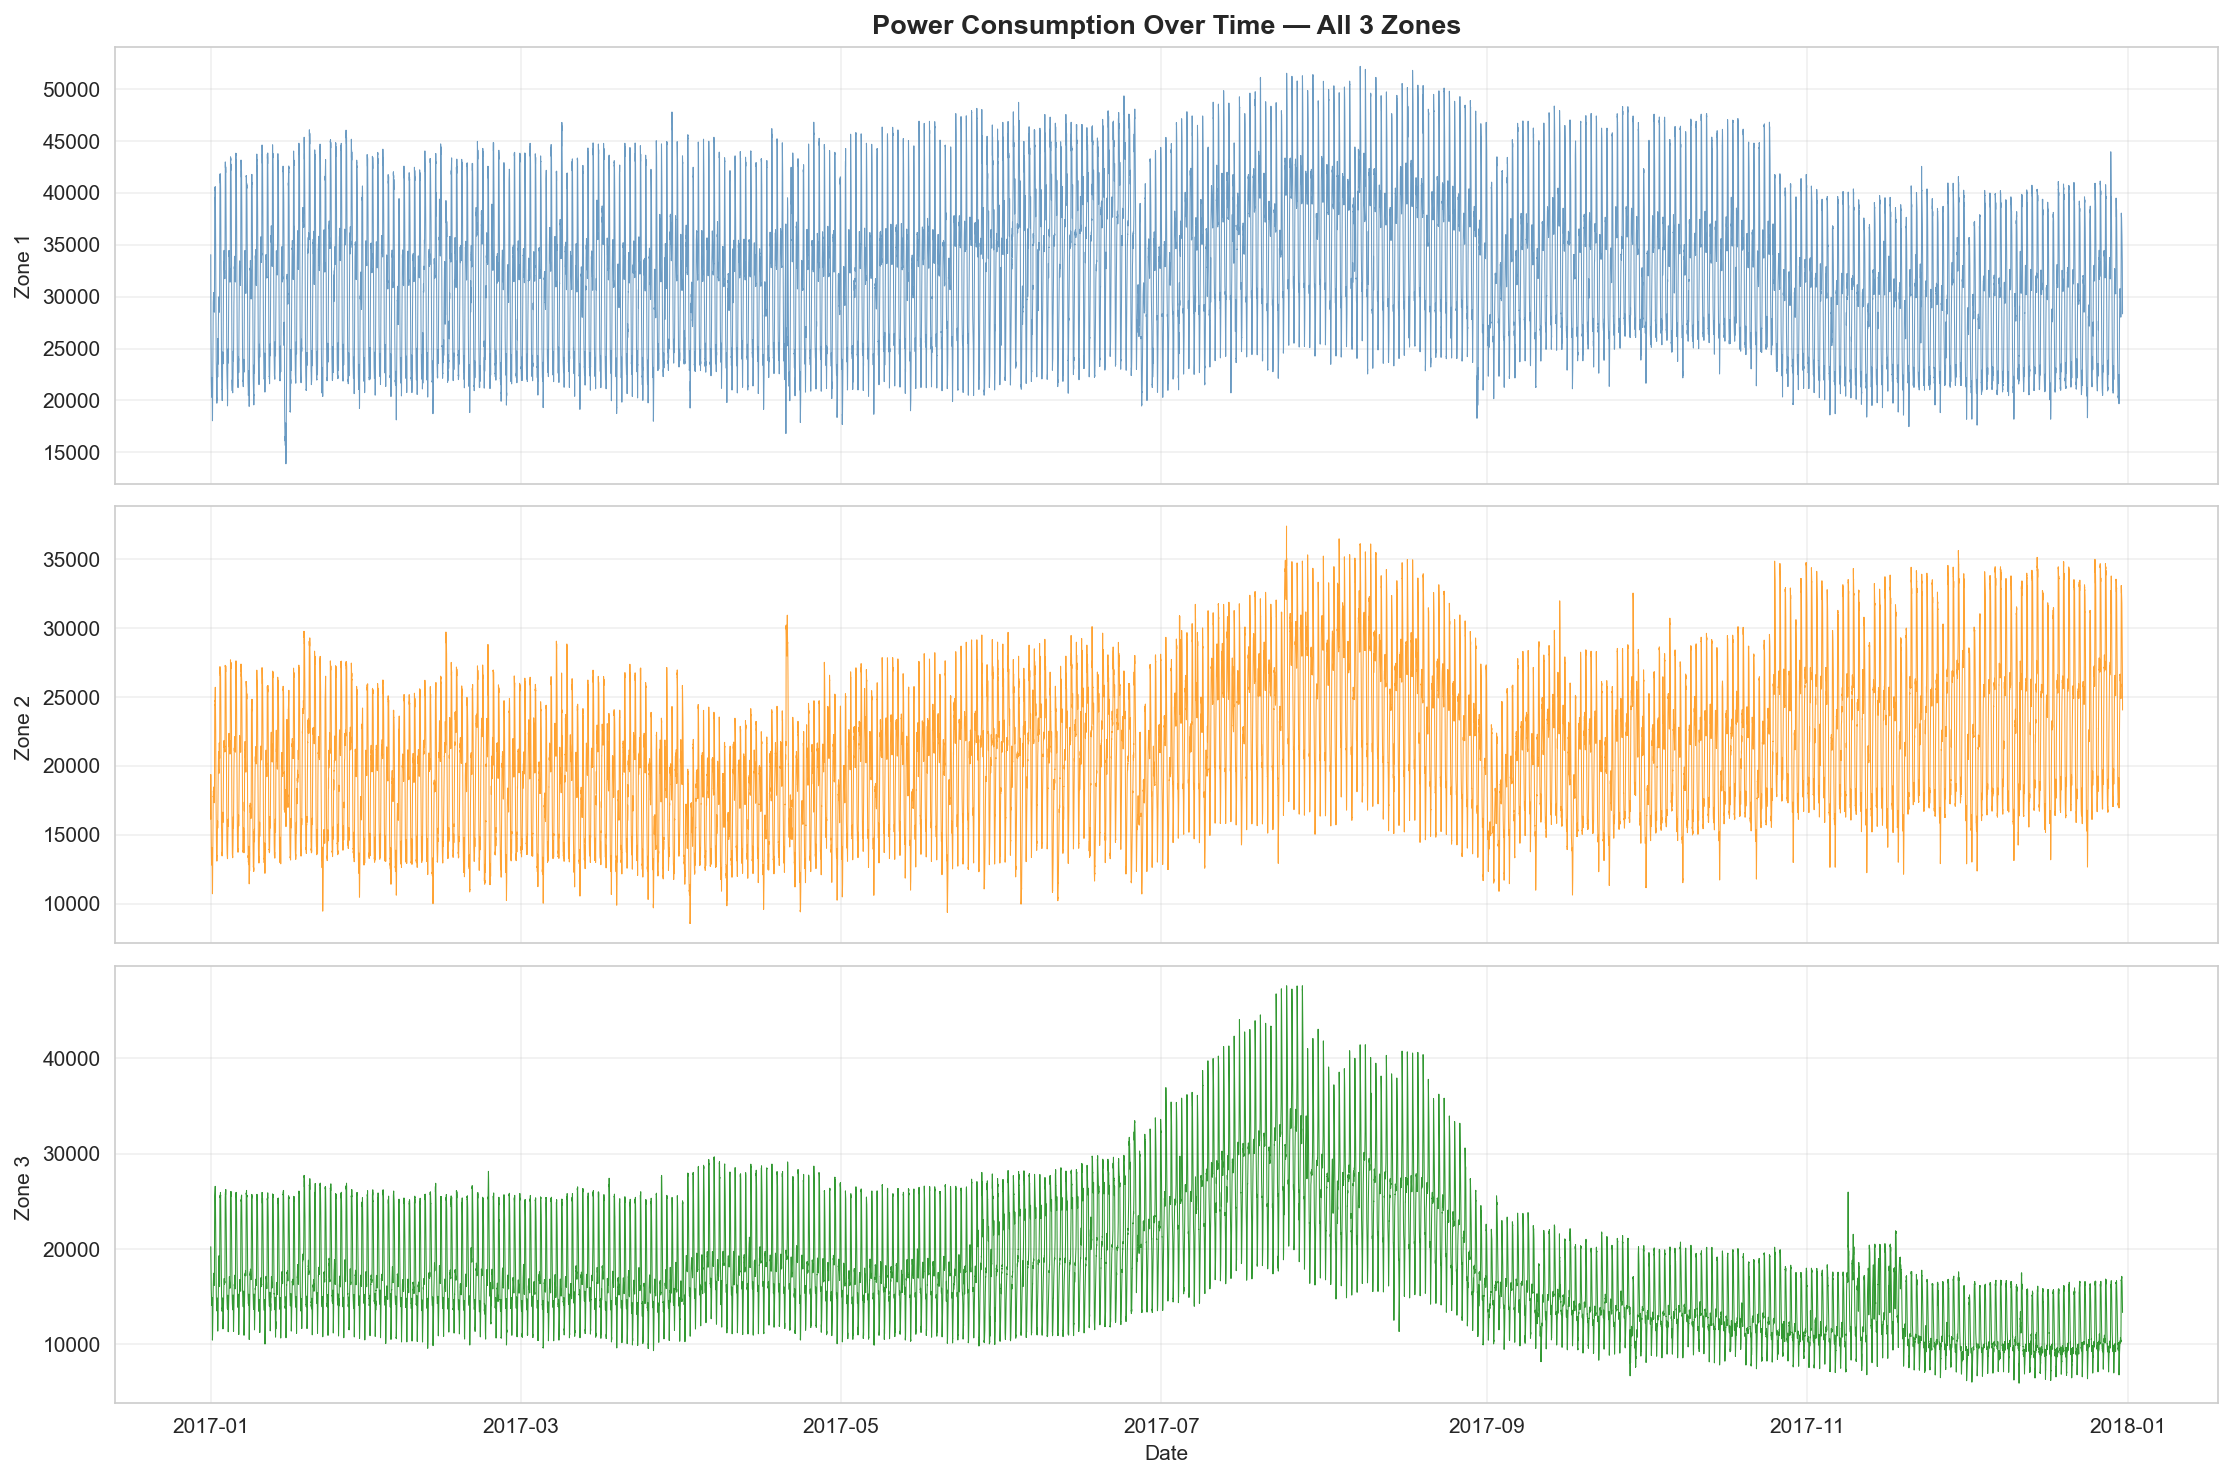
\includegraphics[width=\linewidth,height=3.4cm,keepaspectratio]{plot1_timeseries.png}
  \end{block}
  \vspace{3pt}
  \begin{tikzpicture}
    \node[fill=WarnBg,draw=AccentOrange,rounded corners=3pt,
          inner sep=5pt,text width=\linewidth-4pt]{
      \footnotesize\textcolor{AccentOrange}{\textbf{\faWarning\ Class Imbalance:}}
      \textcolor{DarkText}{Only 0.727\% of readings are outages.
      Standard accuracy is misleading --- \textbf{F1-score} is the correct metric.}
    };
  \end{tikzpicture}
\end{columns}
\end{frame}

%% SLIDE 5 ── EDA ────────────────────────────────────────────
\begin{frame}{Exploratory Data Analysis}
\begin{columns}[t]
\column{0.57\textwidth}
  \begin{block}{Outage Pattern Analysis}
    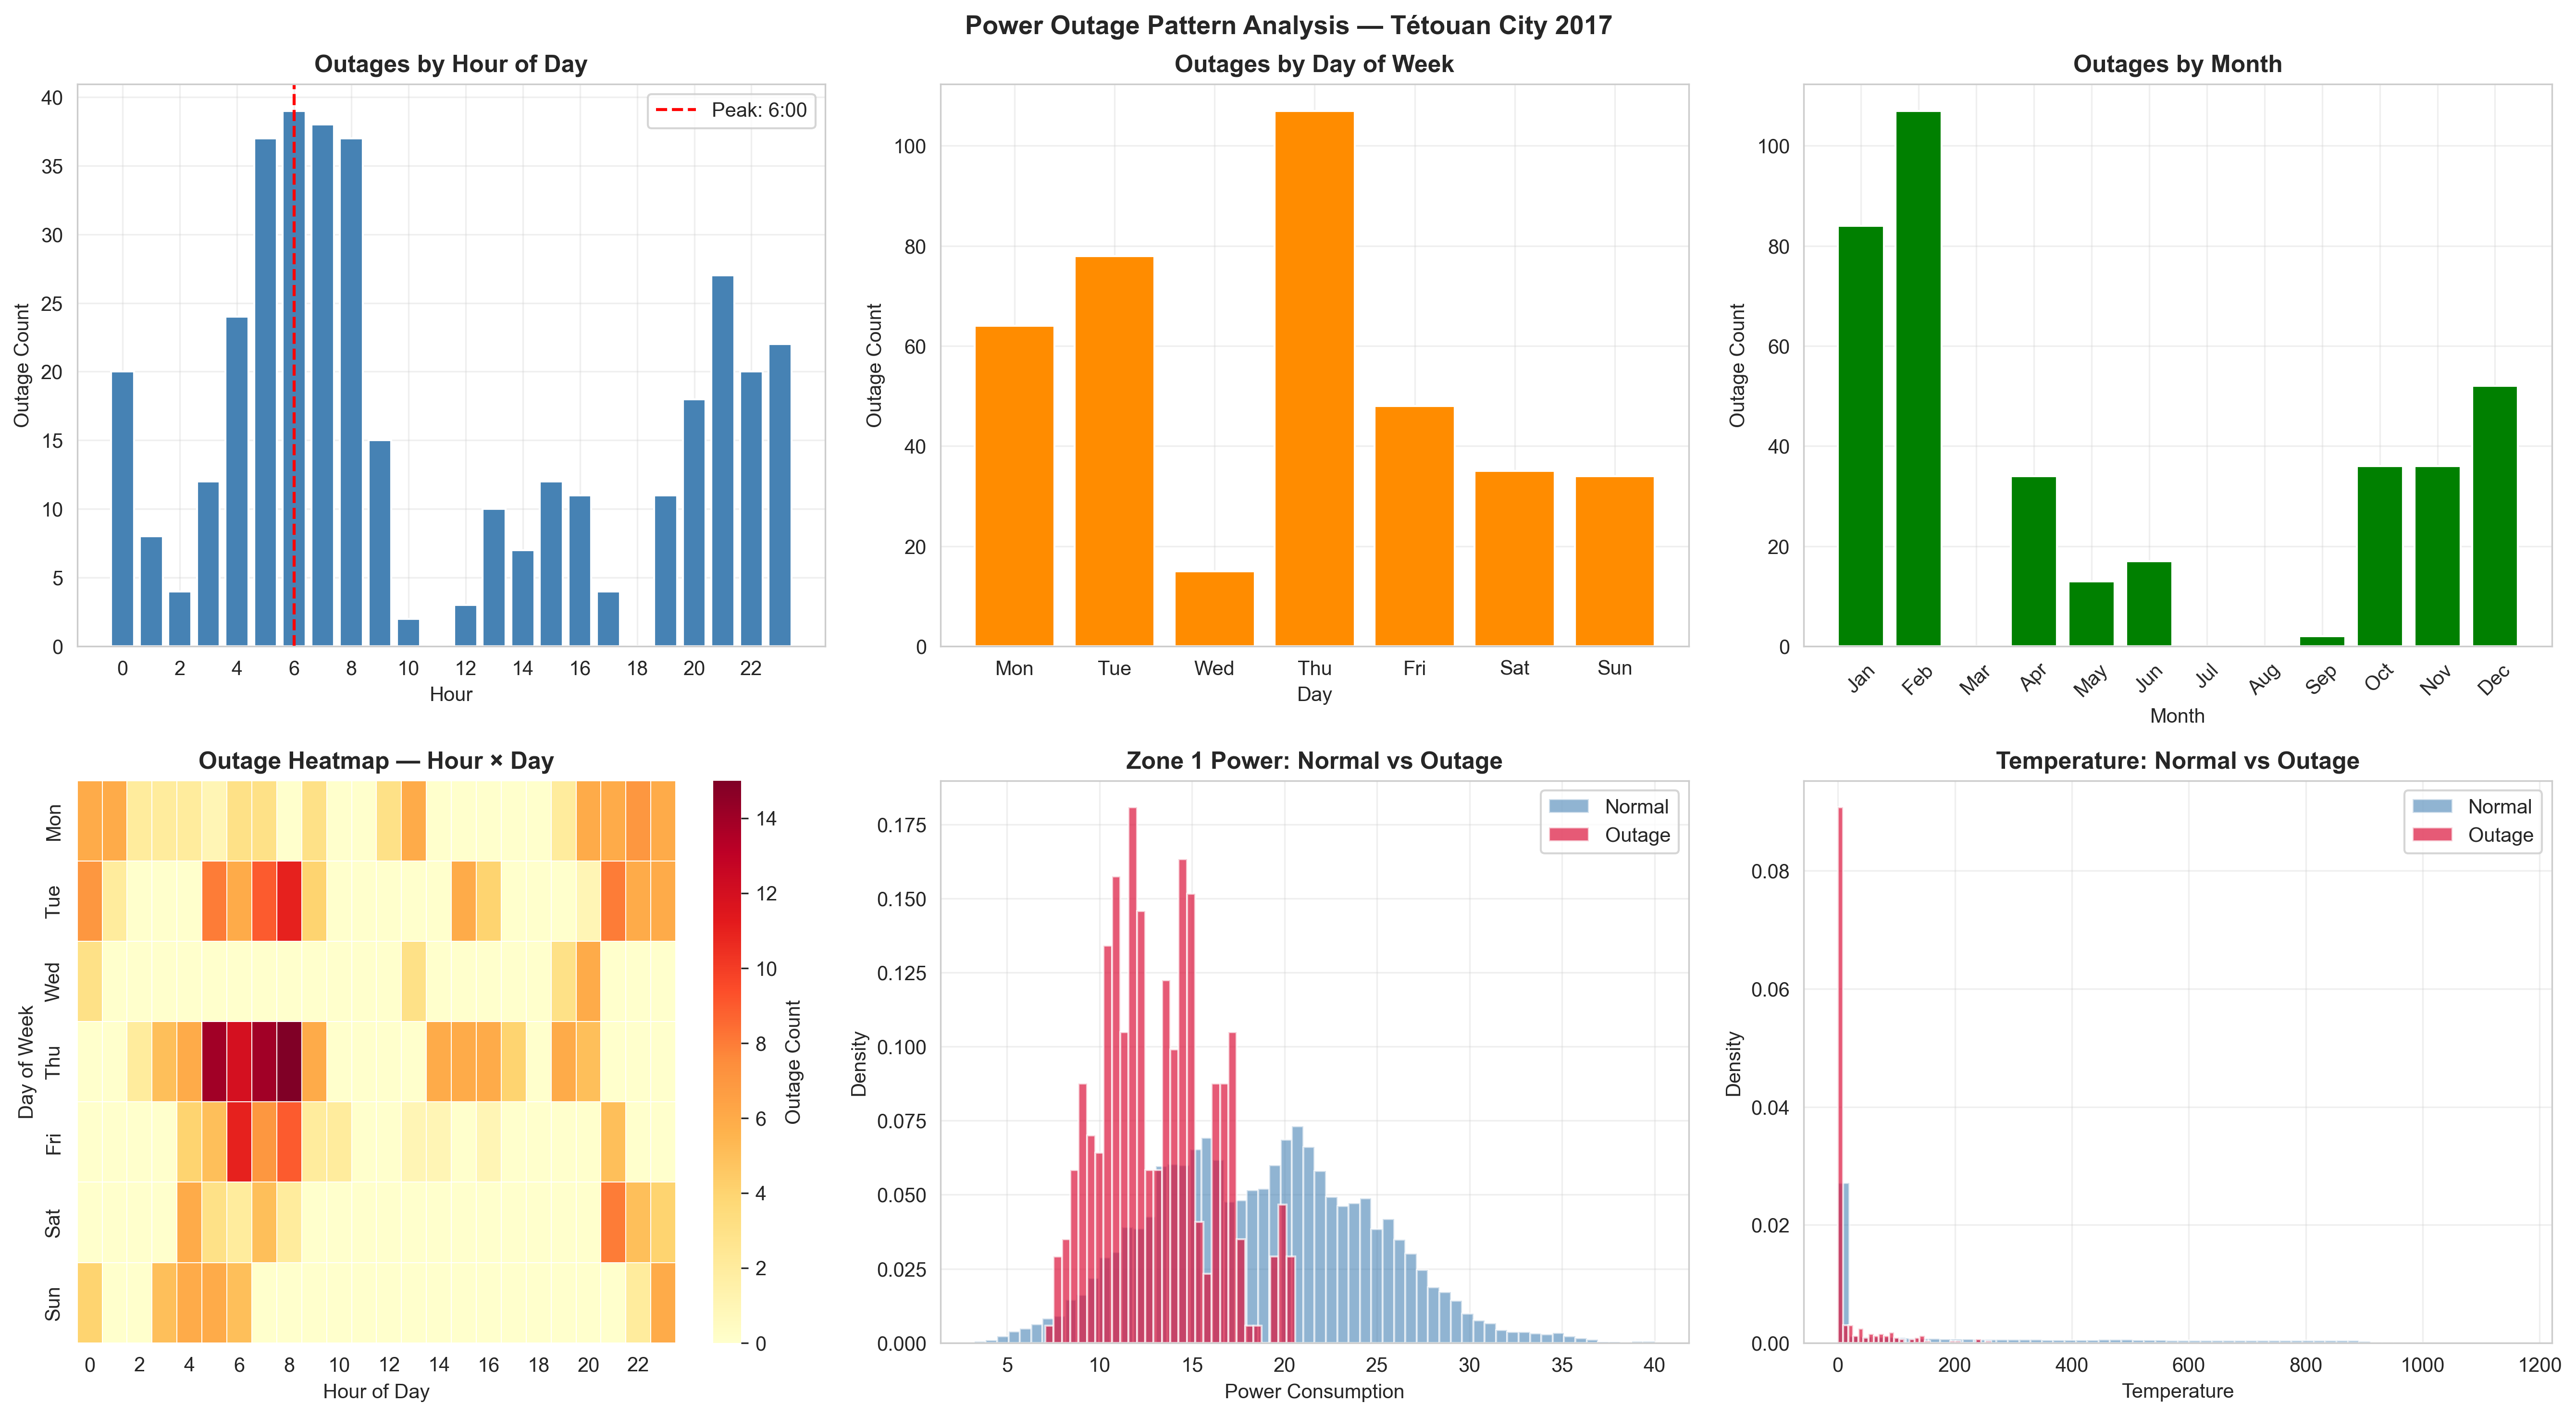
\includegraphics[width=\linewidth,height=4.0cm,keepaspectratio]{day4_plot4_outage_patterns.png}
  \end{block}
\column{0.40\textwidth}
  \begin{exampleblock}{\faKey\ Key Findings}
    \begin{itemize}\setlength\itemsep{3pt}
      \item \textbf{Peak hour:} 6:00 AM\\{\tiny Early-morning load switching}
      \item \textbf{Peak day:} Thursday\\{\tiny Mid-week operational anomaly}
      \item \textbf{Peak month:} February\\{\tiny Winter demand surge}
      \item \textbf{Outage rate:} 0.727\%\\{\tiny Severe class imbalance}
      \item Zone 1 \& 2: $r=-0.460$ (negative)
      \item Zone 1 \& 3: $r=+0.477$ (positive)
    \end{itemize}
  \end{exampleblock}
\end{columns}
\end{frame}

%% SLIDE 6 ── FEATURE ENGINEERING ───────────────────────────
\begin{frame}{Feature Engineering --- 8 Raw $\to$ 39 Features}
\begin{columns}[t]
\column{0.50\textwidth}
  \begin{block}{Feature Categories}
    \footnotesize
    \renewcommand{\arraystretch}{1.2}
    \begin{tabular}{@{}lp{3.5cm}c@{}}
      \toprule
      \textbf{Category} & \textbf{Examples} & \textbf{N}\\
      \midrule
      \rowcolor{RowAlt} Rolling Stats & Mean/std/min/max (2hr,24hr,48hr) & 12\\
      Lag \& Diff     & Lag 1/6/144 steps; diff & 6\\
      \rowcolor{RowAlt} Z-Score       & 24hr z-score, momentum & 2\\
      Time Features   & Hour, day, month, weekend, night & 5\\
      \rowcolor{RowAlt} Interaction   & Zone ratios, weather$\times$power & 9\\
      Raw Features    & Zone 1/2/3, temp, humidity, wind & 5\\
      \midrule
      \textbf{Total}  & & \textbf{39}\\
      \bottomrule
    \end{tabular}
  \end{block}
  \vspace{3pt}
  \begin{tikzpicture}
    \node[fill=CardBg,draw=AccentTeal,rounded corners=3pt,
          inner sep=5pt,text width=\linewidth-4pt]{
      \footnotesize\textcolor{AccentTeal}{\faArrowRight\ \textbf{Top 2 SHAP features:}}
      \textcolor{DarkText}{\texttt{z1\_zscore} (8.456) and \texttt{z1\_rolling\_std\_w144} (0.551)}
    };
  \end{tikzpicture}
\column{0.47\textwidth}
  \begin{block}{Labelled Outage Points}
    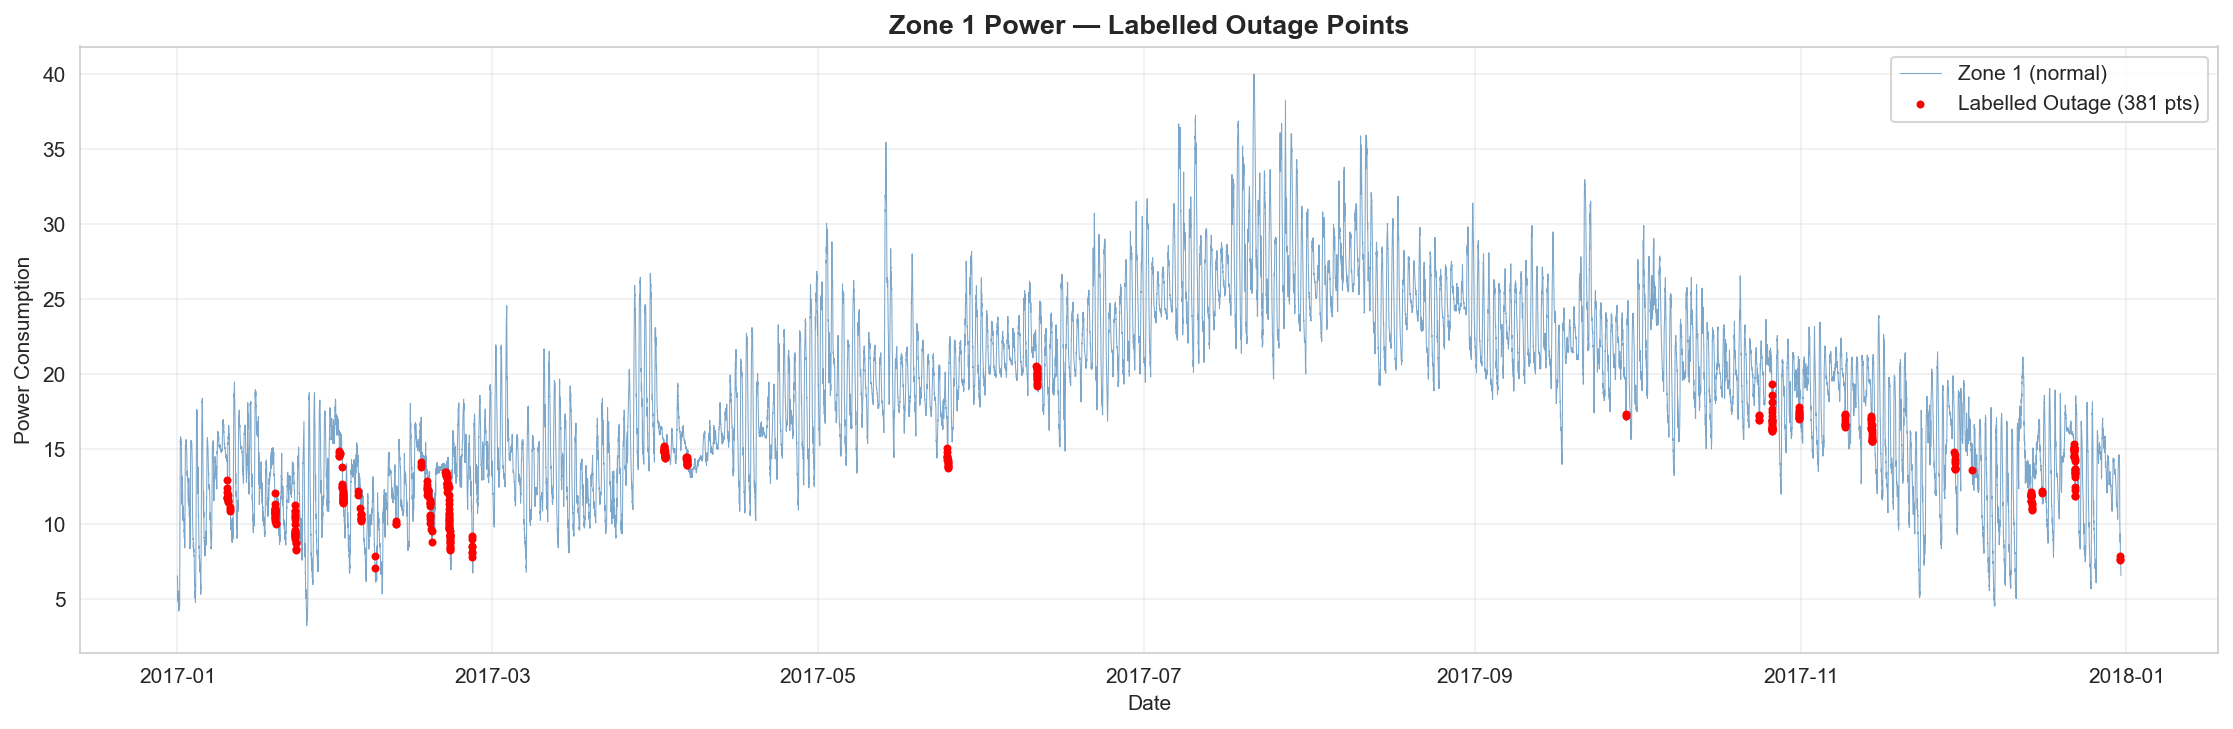
\includegraphics[width=\linewidth,height=2.8cm,keepaspectratio]{plot7_labelled_outages.png}
  \end{block}
  \vspace{3pt}
  \begin{block}{Outage Heatmap (Hour $\times$ Day)}
    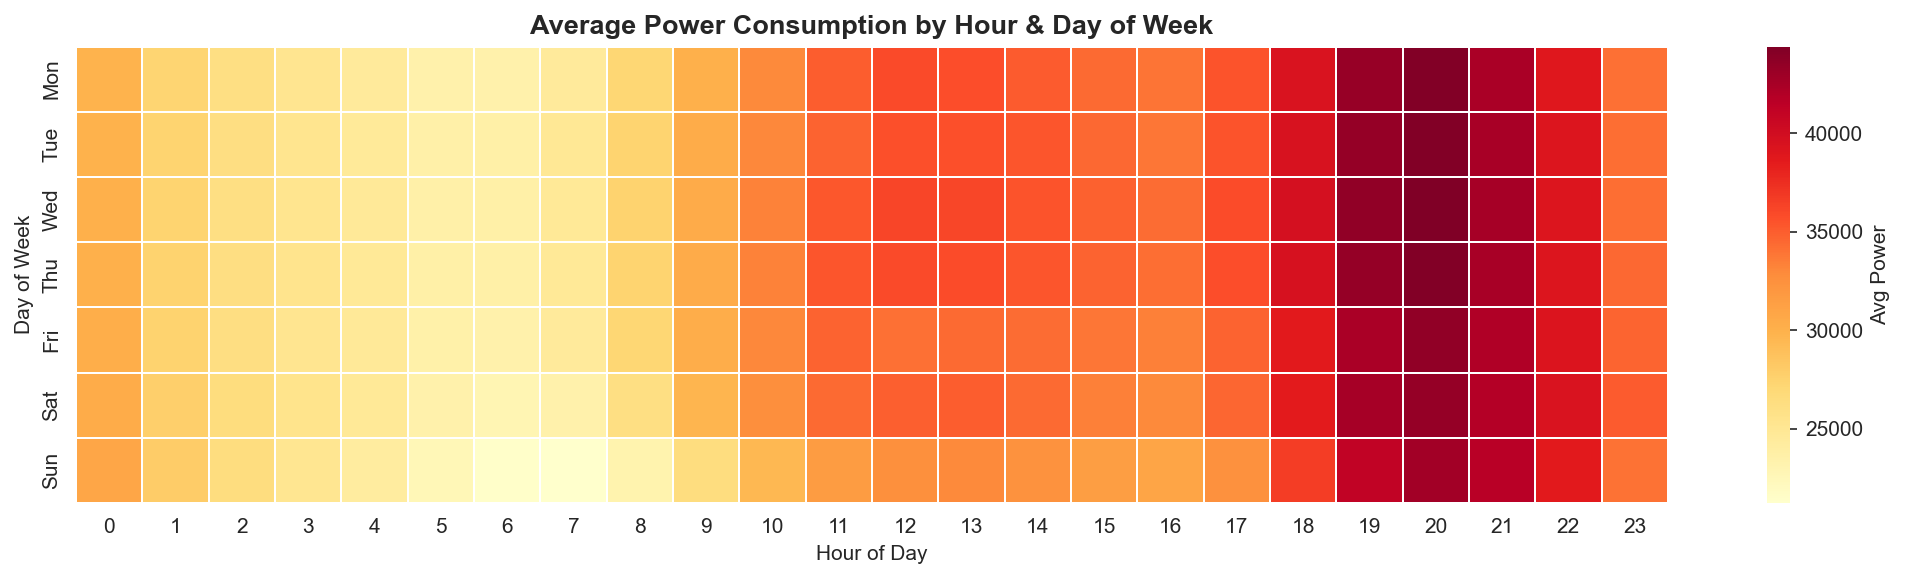
\includegraphics[width=\linewidth,height=2.4cm,keepaspectratio]{plot4_heatmap.png}
  \end{block}
\end{columns}
\end{frame}

%% SLIDE 7 ── MODELS ─────────────────────────────────────────
\begin{frame}{Models Evaluated --- 6 Models, 2 Paradigms}
\begin{columns}[t]
\column{0.48\textwidth}
  \begin{block}{\faTag\ Supervised (with labels)}
    \footnotesize
    \begin{itemize}\setlength\itemsep{3pt}
      \item \textbf{Logistic Regression} --- linear baseline
      \item \textbf{Decision Tree} --- rule-based baseline
      \item \textbf{Random Forest} --- ensemble baseline
      \item \textbf{Neural Network} --- Giant arch\\
            (1024-512-256-128-64-32), 500 epochs,\\
            cosine LR annealing, 20 training runs
      \item \hl{XGBoost\ \faTrophy\ Champion} ---\\
            2000-tree ceiling, early stop at round 164
    \end{itemize}
  \end{block}
\column{0.48\textwidth}
  \begin{block}{\faMagic\ Unsupervised (no labels needed)}
    \footnotesize
    \begin{itemize}\setlength\itemsep{3pt}
      \item \textbf{Isolation Forest} --- random splits to isolate anomalies; 5 contamination values tuned
      \item \textbf{LSTM Autoencoder} --- learns normal 8-hour consumption patterns; flags sequences with high reconstruction error
    \end{itemize}
  \end{block}
  \vspace{3pt}
  \begin{exampleblock}{\faInfoCircle\ Why Both Paradigms?}
    \footnotesize
    Supervised needs labels.
    Unsupervised works when labelling every outage is expensive or infeasible in real deployments.
  \end{exampleblock}
\end{columns}
\end{frame}

%% SLIDE 8 ── ARCHITECTURE TOURNAMENT ────────────────────────
\begin{frame}{Neural Network --- Architecture Tournament}
\begin{columns}[t]
\column{0.55\textwidth}
  \begin{block}{Tournament Results (5-Fold CV)}
    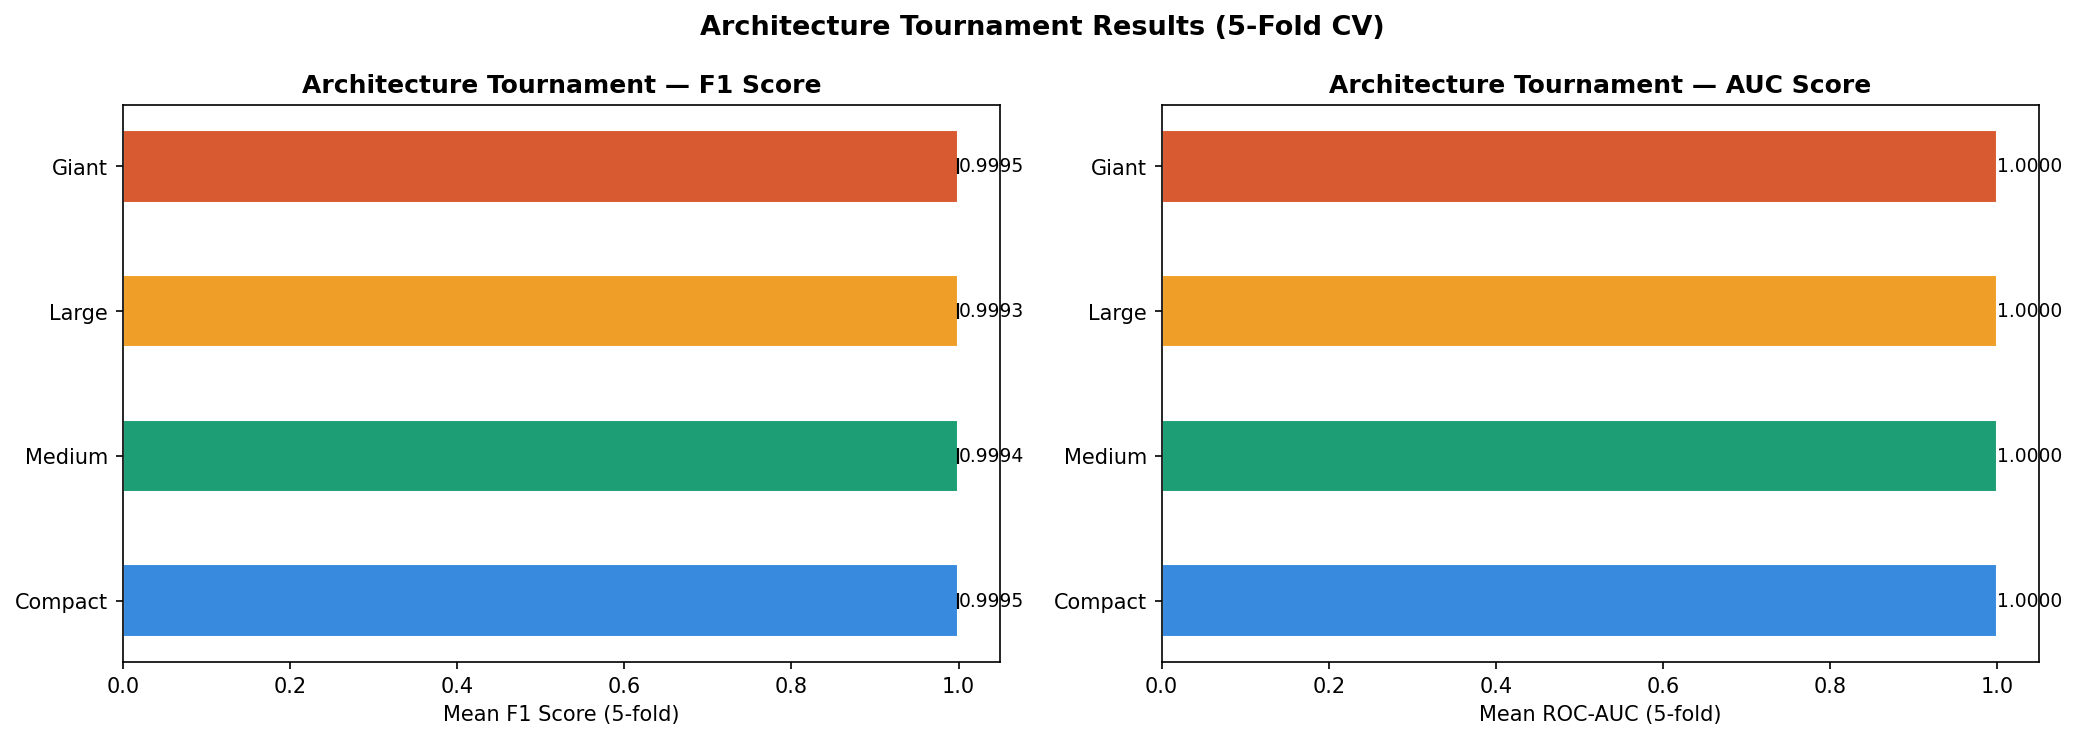
\includegraphics[width=\linewidth,height=3.2cm,keepaspectratio]{plot_tournament.png}
  \end{block}
  \vspace{2pt}
  \begin{block}{Final Model Training Curves}
    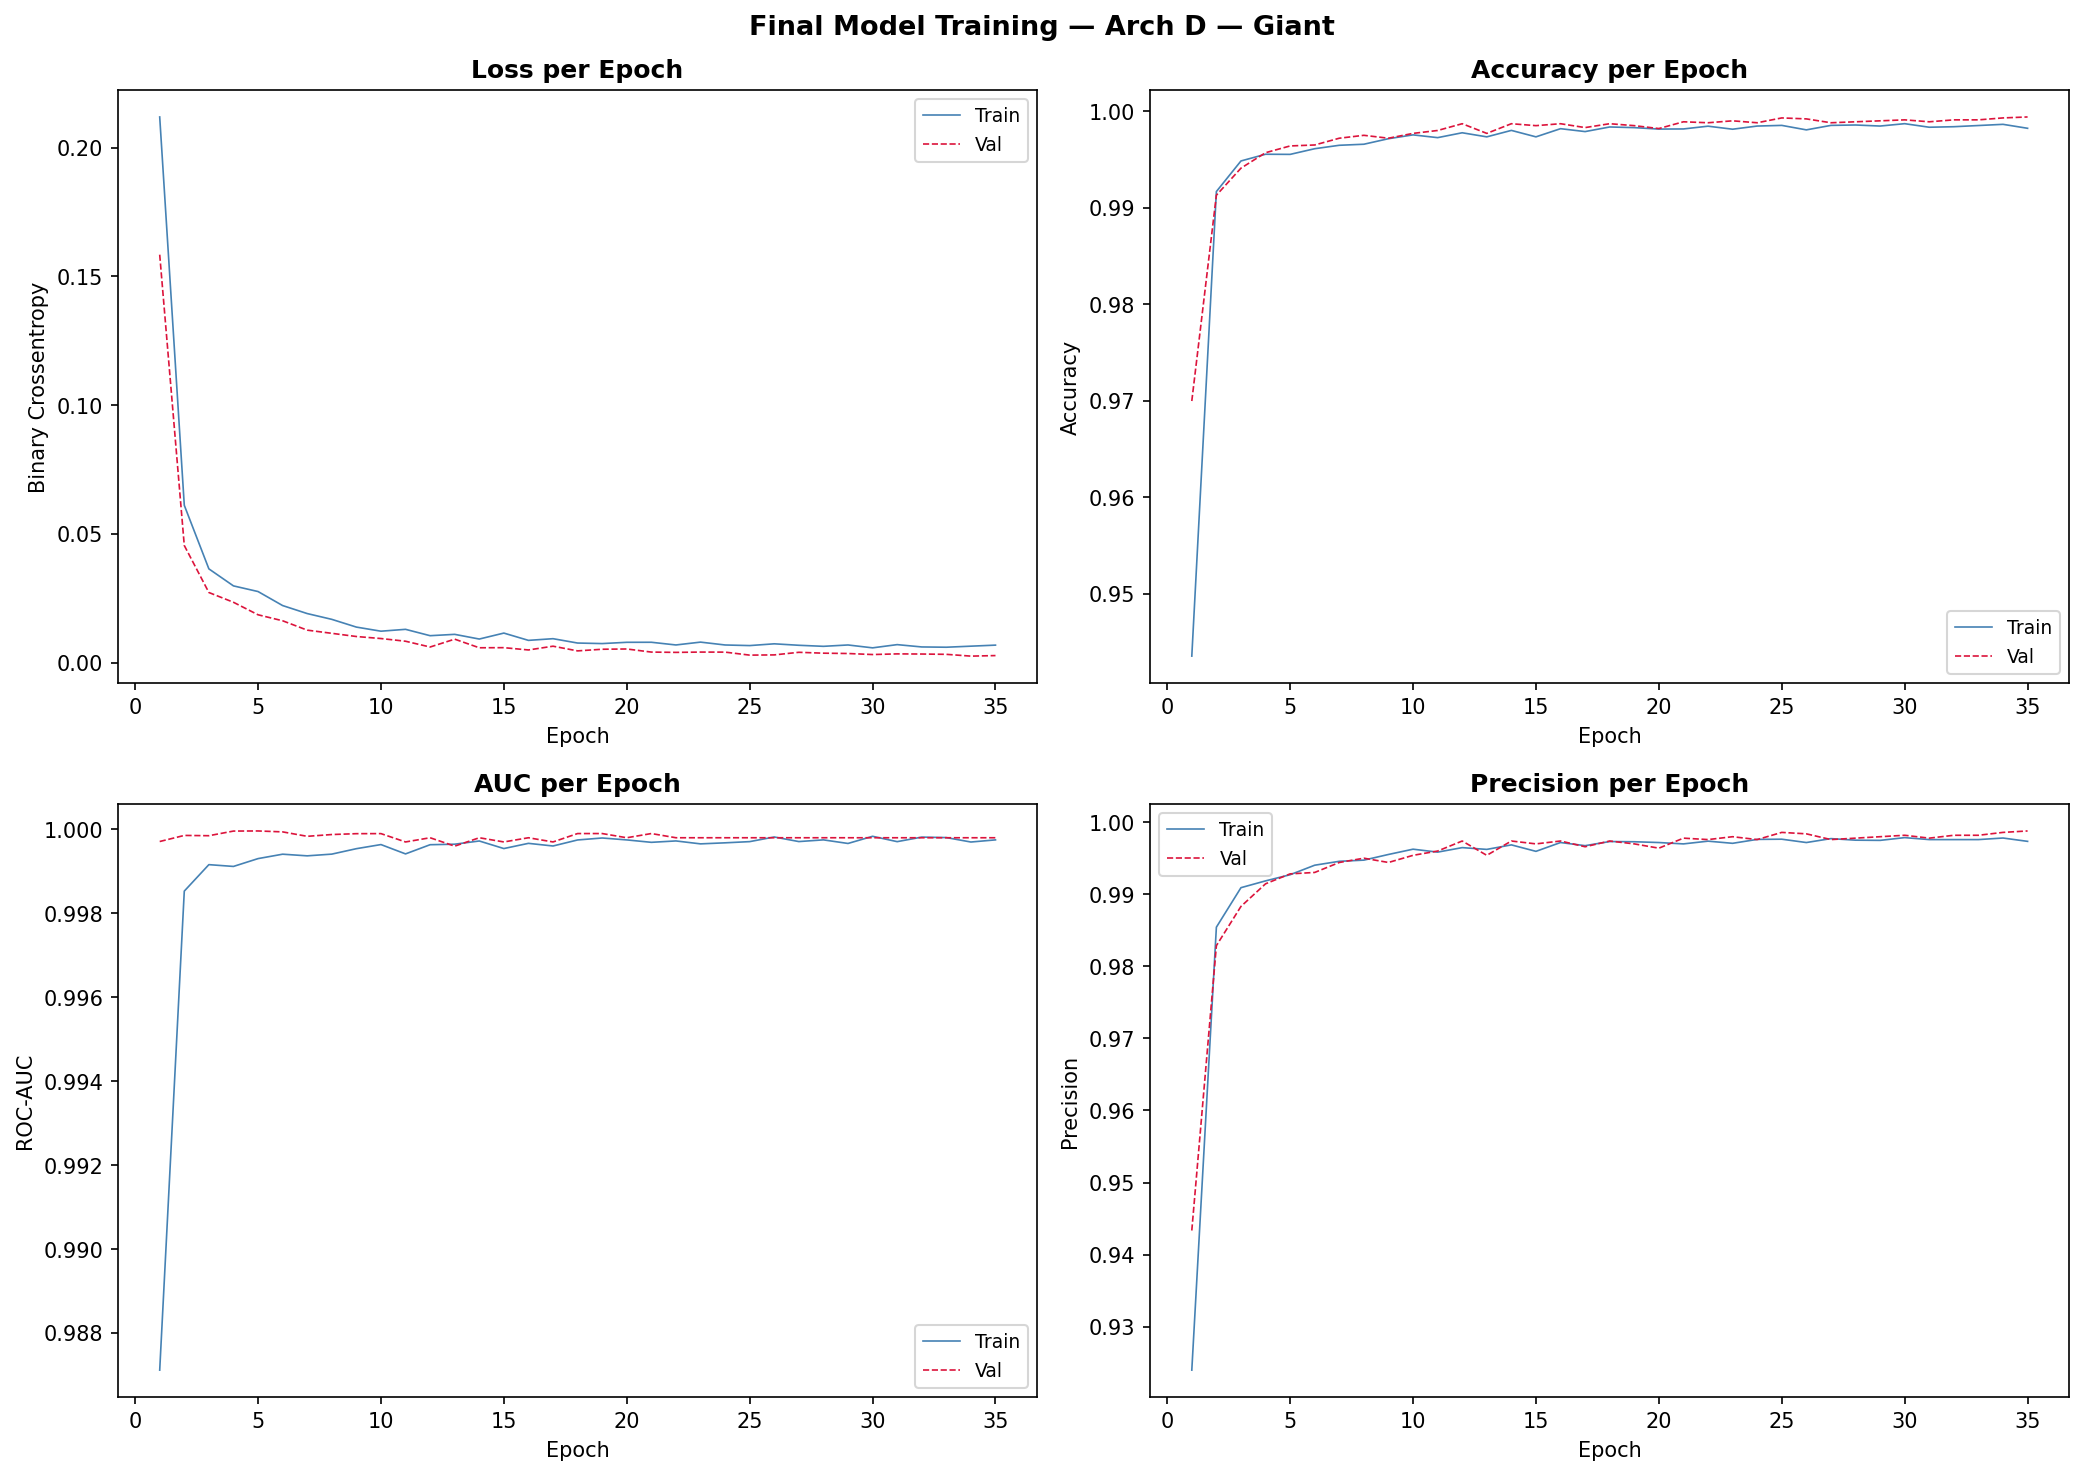
\includegraphics[width=\linewidth,height=2.3cm,keepaspectratio]{plot_final_training_curves.png}
  \end{block}
\column{0.42\textwidth}
  \begin{alertblock}{\faTrophy\ Winner: Giant Arch}
    \footnotesize\texttt{1024-512-256-128-64-32}
  \end{alertblock}
  \vspace{3pt}
  \footnotesize
  \renewcommand{\arraystretch}{1.2}
  \begin{tabular}{@{}ll@{}}
    \toprule
    \textbf{Setting} & \textbf{Value}\\
    \midrule
    \rowcolor{RowAlt} Architectures & 4\\
    CV Folds        & 5\\
    \rowcolor{RowAlt} Training Runs & \textbf{20}\\
    Max Epochs      & 500\\
    \rowcolor{RowAlt} Learning Rate & 0.0001\\
    LR Schedule     & Cosine Anneal\\
    \rowcolor{RowAlt} Early Stop    & patience=30\\
    Epochs Ran      & 195\\
    \bottomrule
  \end{tabular}
  \vspace{3pt}
  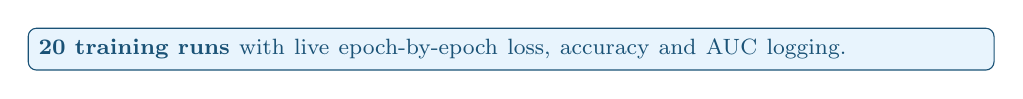
\begin{tikzpicture}
    \node[fill=CardBg,draw=PrimaryBlue,rounded corners=3pt,
          inner sep=4pt,text width=\linewidth-4pt]{
      \footnotesize\textcolor{PrimaryBlue}{\textbf{20 training runs} with live epoch-by-epoch loss, accuracy and AUC logging.}
    };
  \end{tikzpicture}
\end{columns}
\end{frame}

%% SLIDE 9 ── XGBOOST ────────────────────────────────────────
\begin{frame}{XGBoost --- Champion Model}
\begin{columns}[t]
\column{0.55\textwidth}
  \begin{block}{Boosting Rounds --- Logloss Curve}
    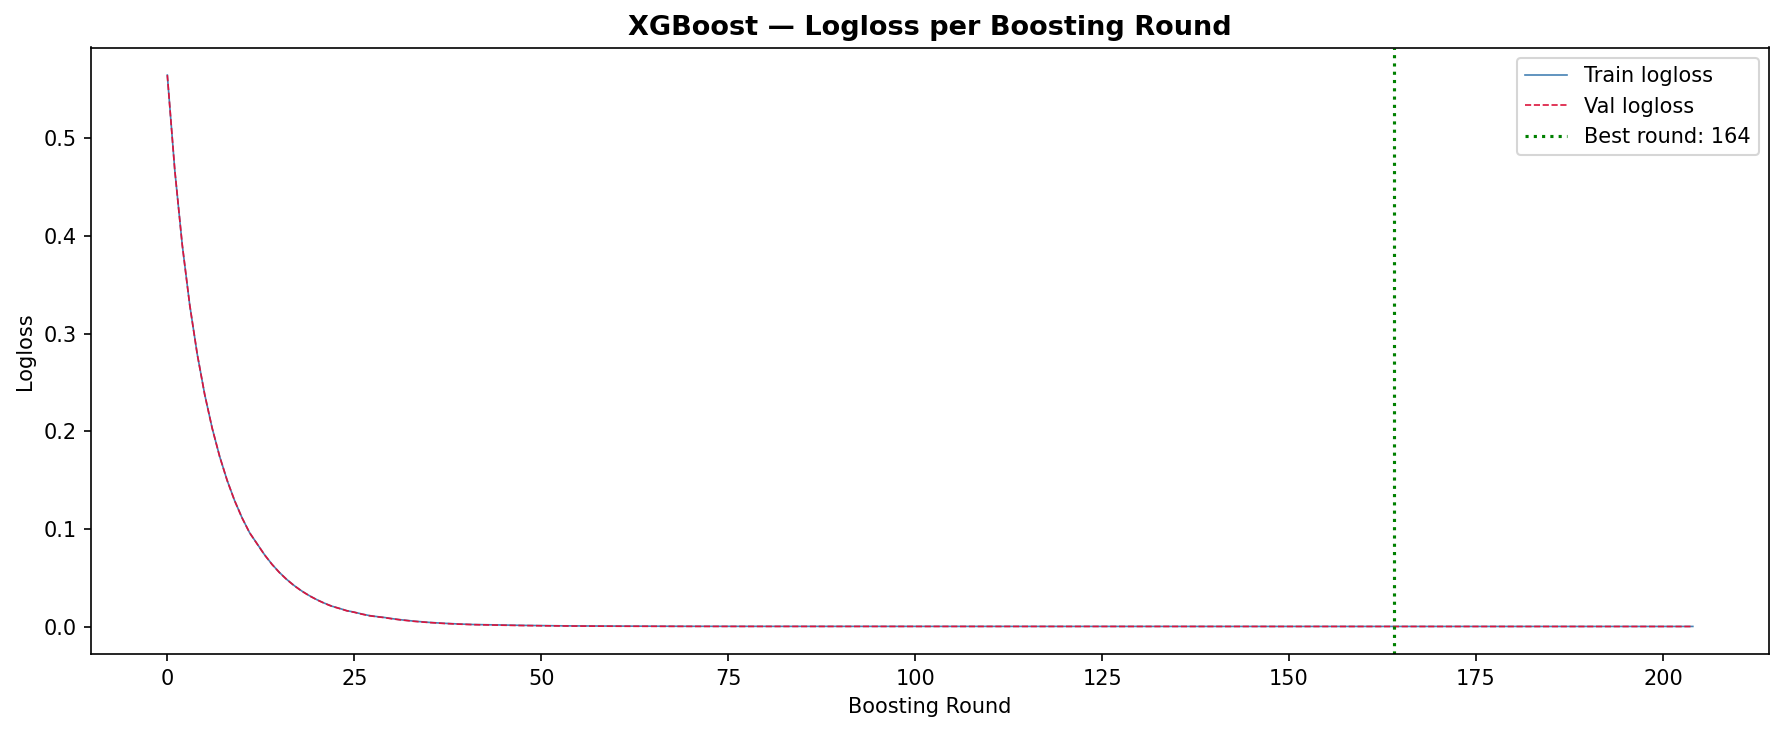
\includegraphics[width=\linewidth,height=3.0cm,keepaspectratio]{plot_xgb_rounds.png}
  \end{block}
  \vspace{2pt}
  \begin{block}{Grand Final Confusion Matrices}
    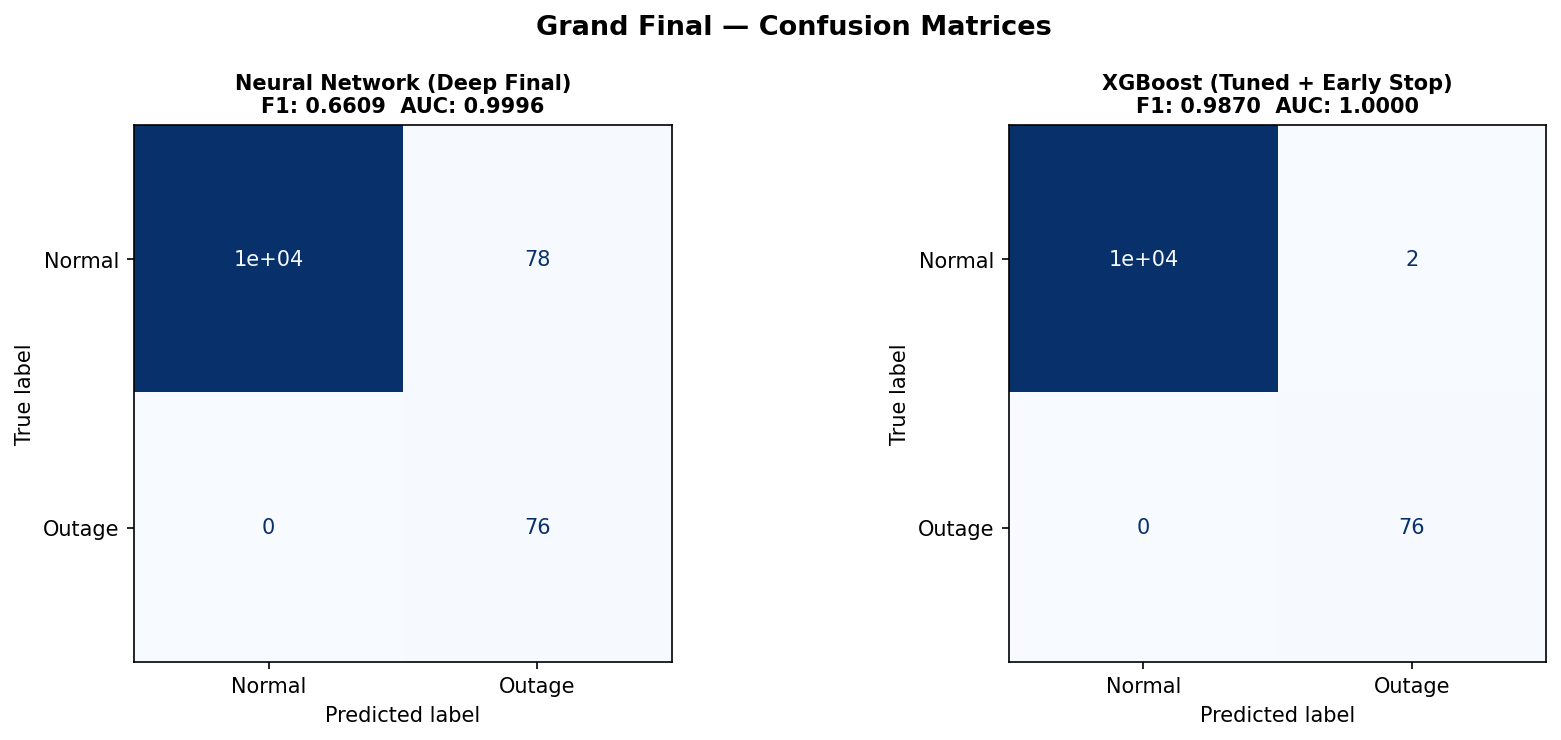
\includegraphics[width=\linewidth,height=2.5cm,keepaspectratio]{plot_grand_final.png}
  \end{block}
\column{0.42\textwidth}
  \begin{exampleblock}{\faChartLine\ Training Setup}
    \footnotesize
    \begin{itemize}\setlength\itemsep{3pt}
      \item RandomizedSearchCV:\\
            30 combos $\times$ 5-fold = \textbf{150 fits}
      \item 2000-tree ceiling\\
            \textbf{early stop at round 164}
      \item Histogram tree method\\
            for CPU efficiency
    \end{itemize}
  \end{exampleblock}
  \vspace{4pt}
  \centering
  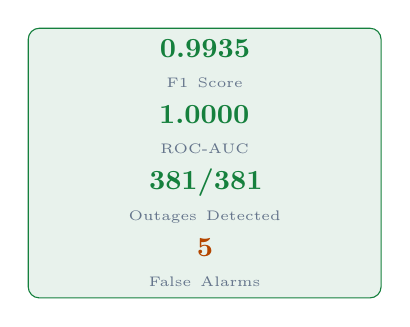
\begin{tikzpicture}
    \node[fill=GreenOk!10,draw=GreenOk,rounded corners=4pt,
          inner sep=4pt,text width=4.2cm,align=center]{
      {\normalsize\bfseries\textcolor{GreenOk}{0.9935}}\\[-1pt]
      {\tiny\textcolor{MutedText}{F1 Score}}\\[1pt]
      {\normalsize\bfseries\textcolor{GreenOk}{1.0000}}\\[-1pt]
      {\tiny\textcolor{MutedText}{ROC-AUC}}\\[1pt]
      {\normalsize\bfseries\textcolor{GreenOk}{381/381}}\\[-1pt]
      {\tiny\textcolor{MutedText}{Outages Detected}}\\[1pt]
      {\normalsize\bfseries\textcolor{AccentOrange}{5}}\\[-1pt]
      {\tiny\textcolor{MutedText}{False Alarms}}
    };
  \end{tikzpicture}
\end{columns}
\end{frame}

%% SLIDE 10 ── SUPERVISED vs UNSUPERVISED ────────────────────
\begin{frame}{Supervised vs.\ Unsupervised Detection}
\begin{block}{January 2017 Detection Window --- Ground Truth vs XGBoost vs Isolation Forest}
  \centering
  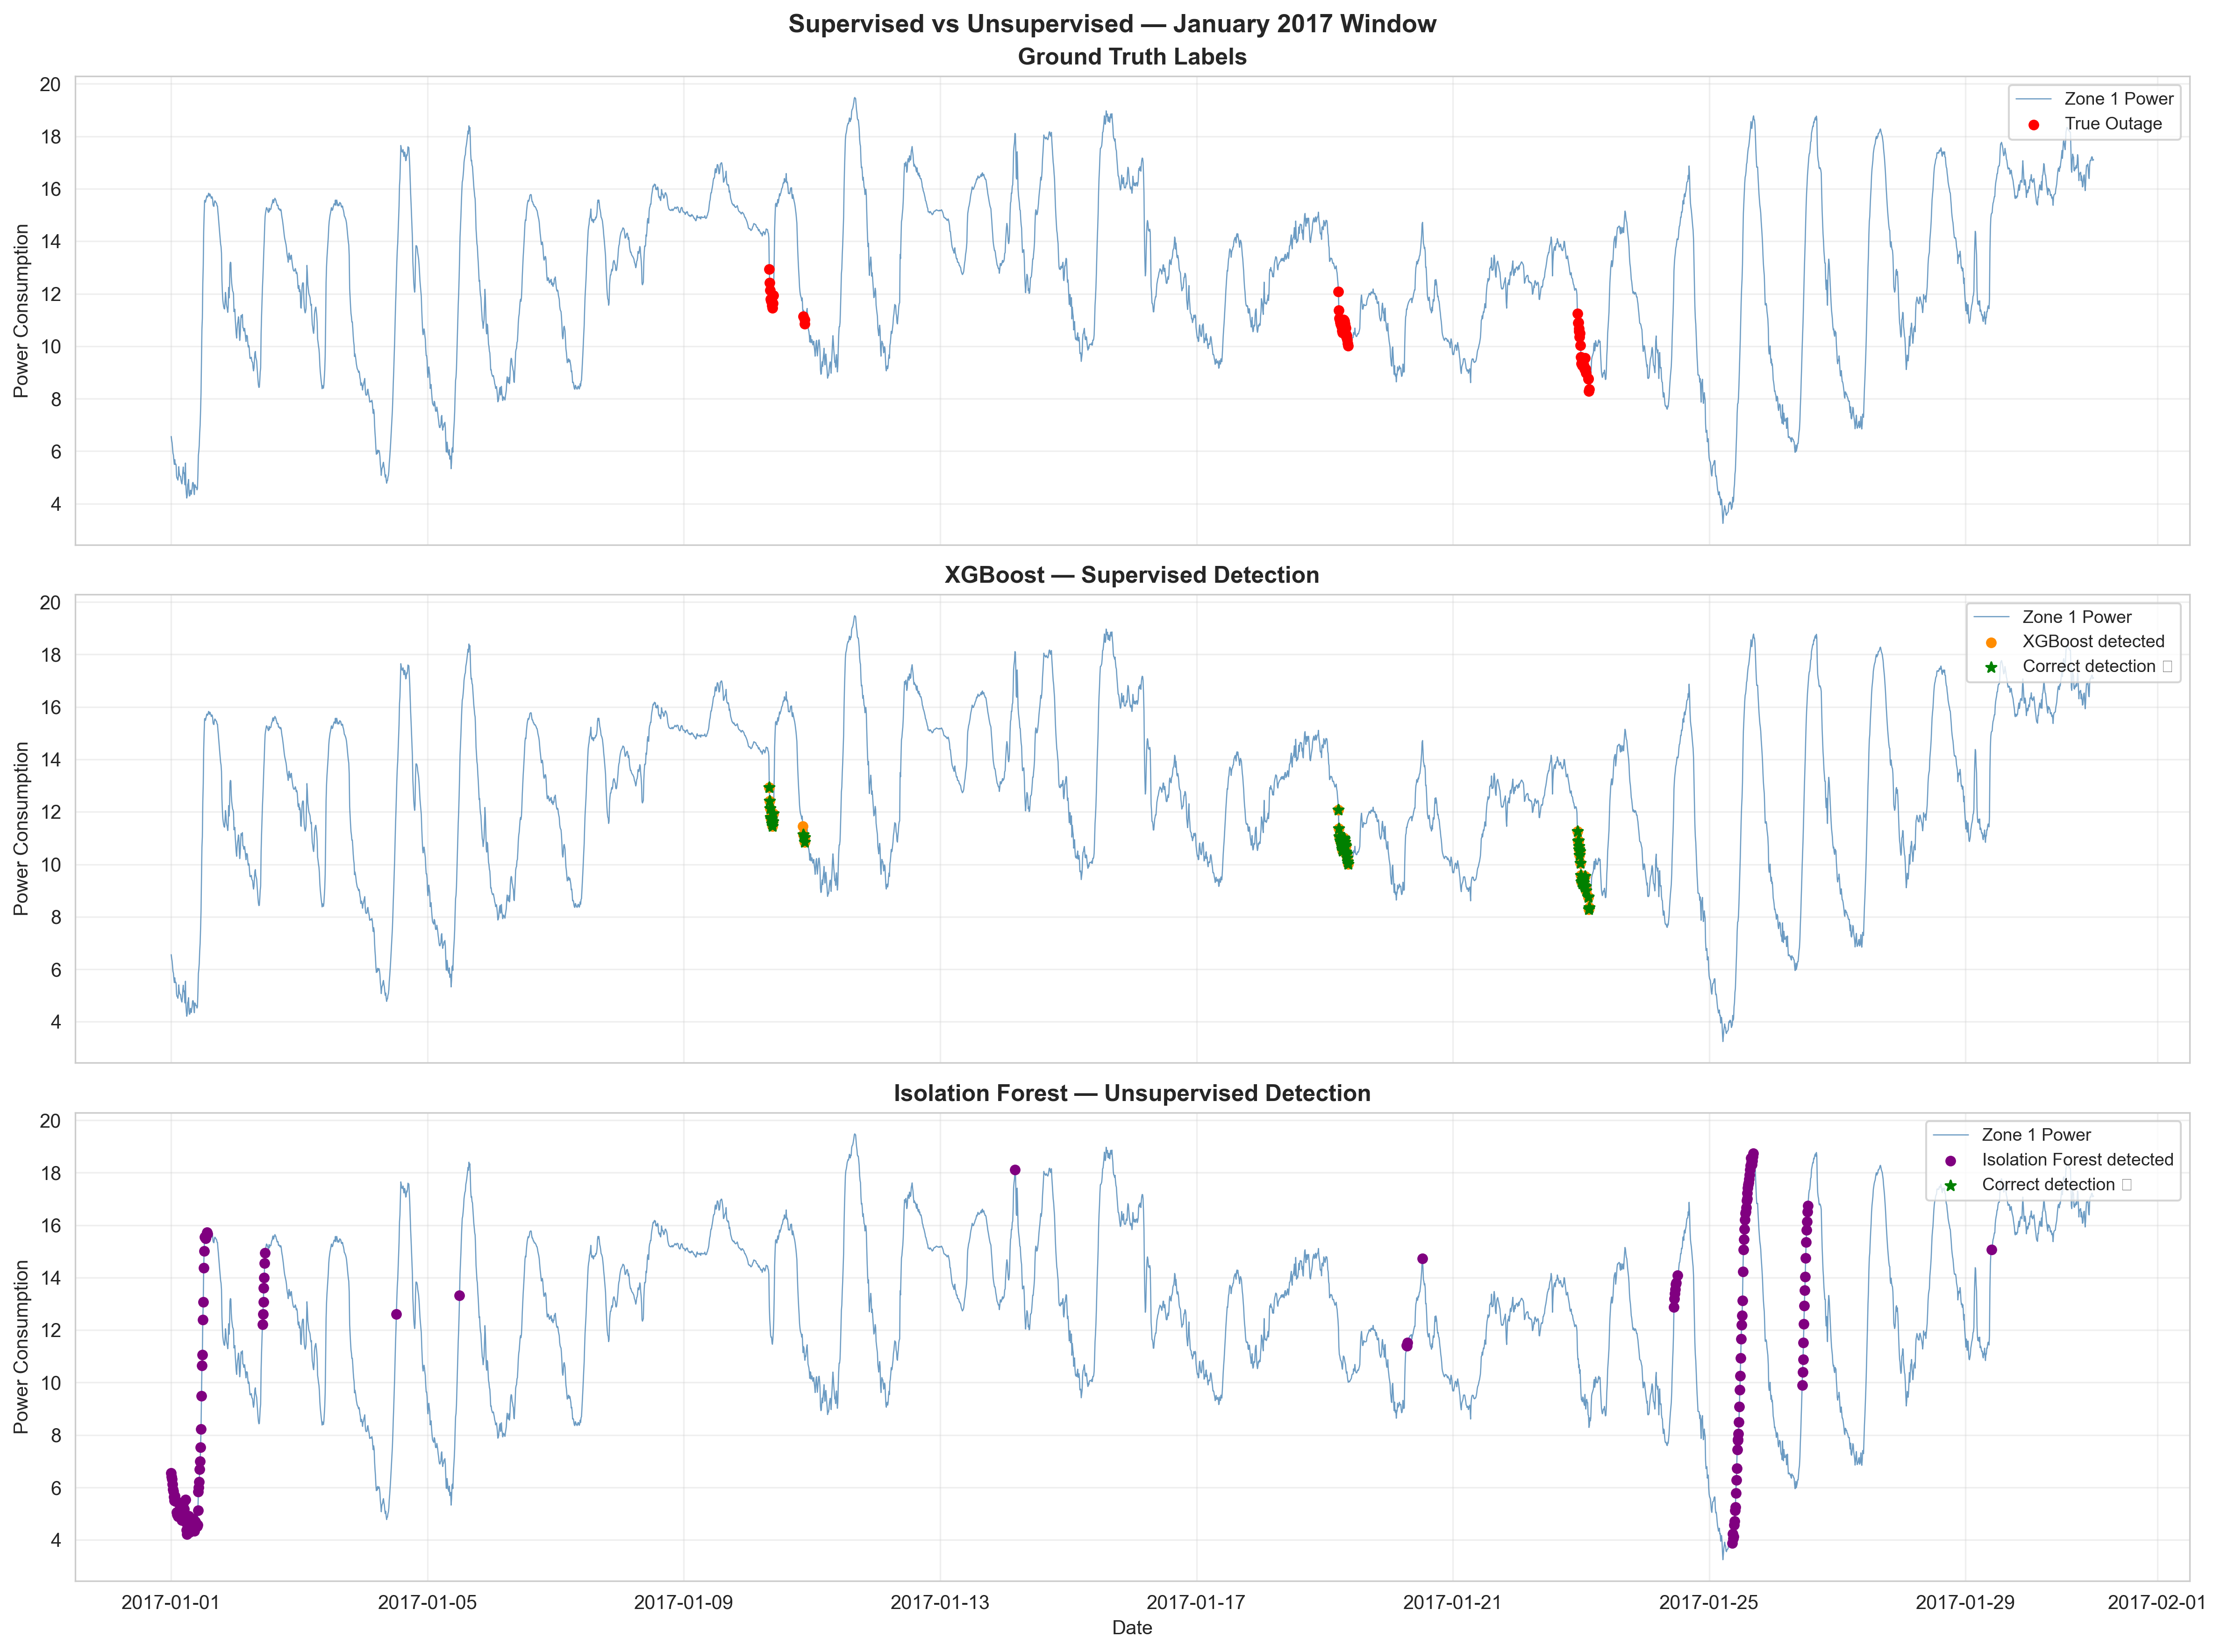
\includegraphics[width=0.92\linewidth,height=4.8cm,keepaspectratio]{day4_plot3_supervised_vs_unsupervised.png}
\end{block}
\vspace{3pt}
\begin{columns}[t]
\column{0.48\textwidth}
  \chip{XGBoost}{GreenOk}\ Needs labels. Learns exact outage signatures.\ \textbf{F1: 0.9935}
\column{0.48\textwidth}
  \chip{Isolation Forest}{AccentOrange}\ No labels needed. Point-level anomaly scores.\ \textbf{F1: 0.0007}
\end{columns}
\end{frame}

%% SLIDE 11 ── ISOLATION FOREST ─────────────────────────────
\begin{frame}{Isolation Forest --- Unsupervised Baseline}
\begin{columns}[t]
\column{0.58\textwidth}
  \begin{block}{Contamination Tuning (5 values)}
    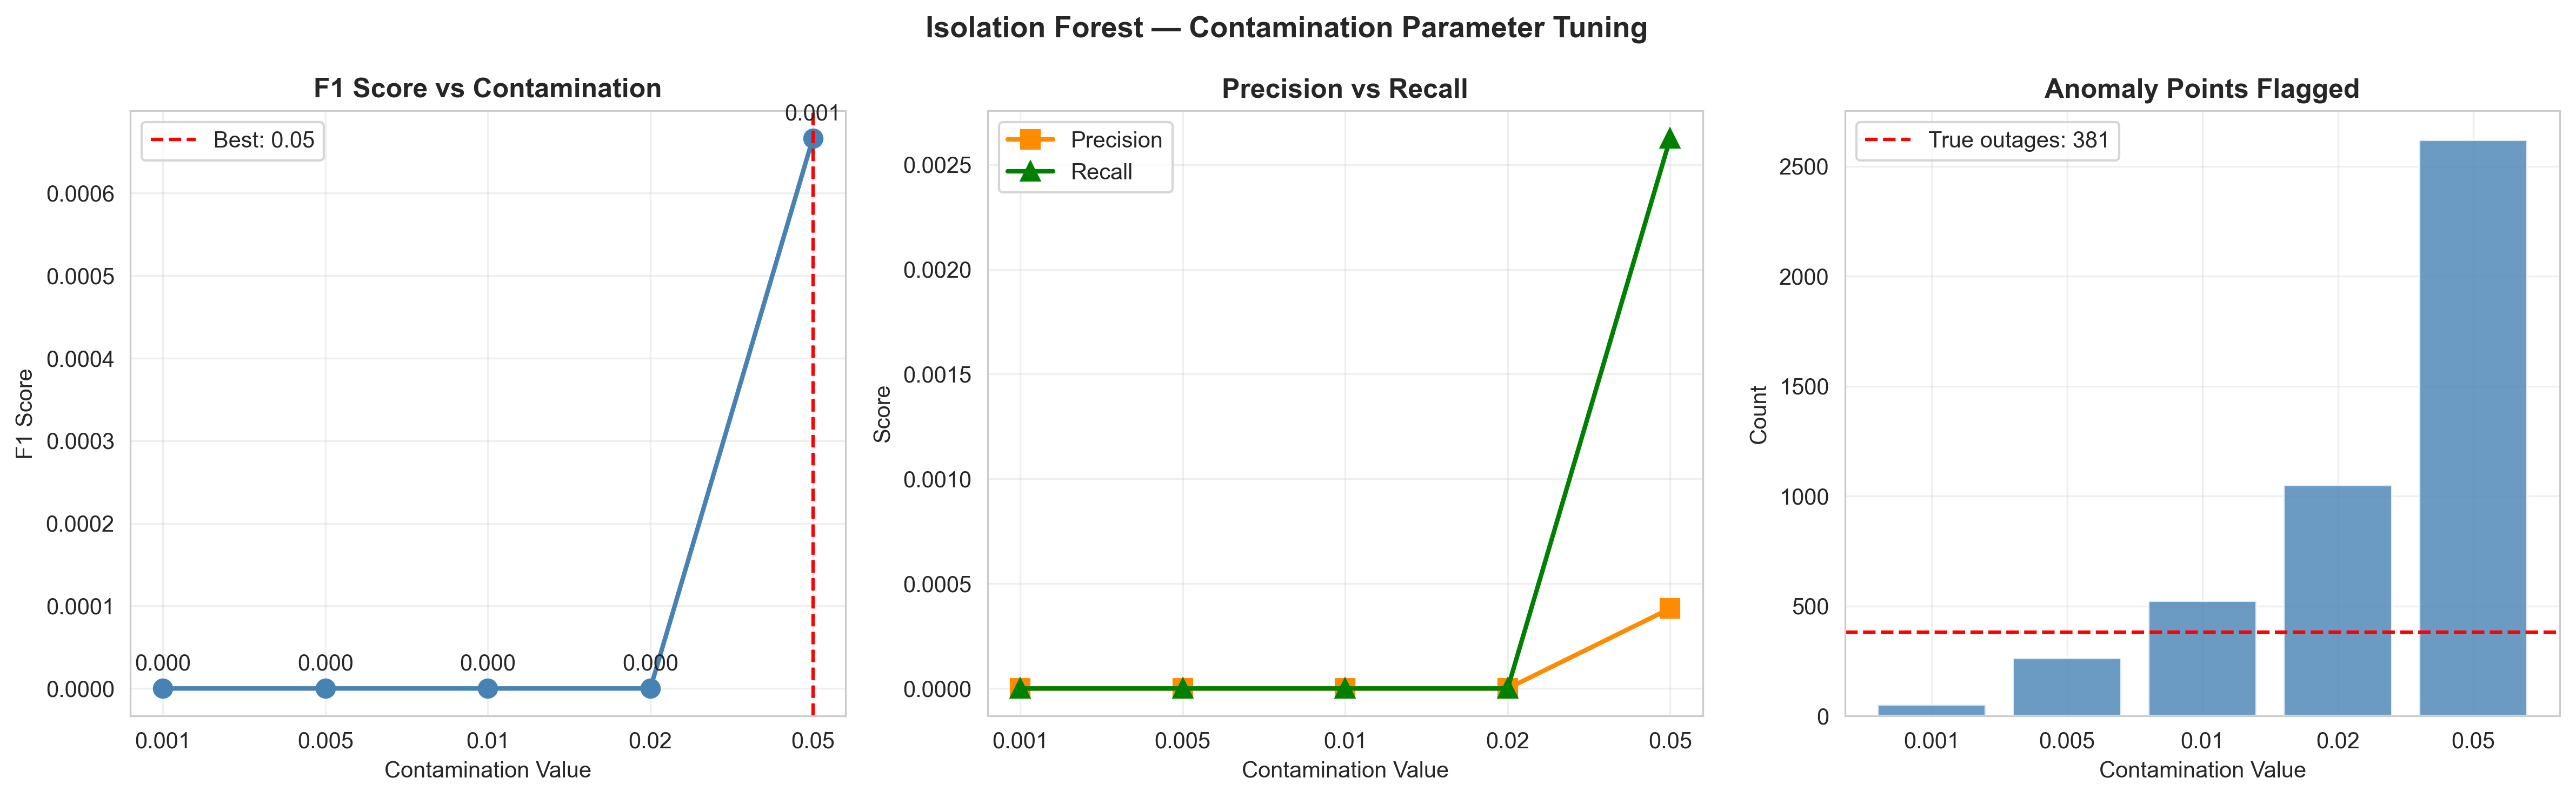
\includegraphics[width=\linewidth,height=2.7cm,keepaspectratio]{day4_plot1_contamination_tuning.png}
  \end{block}
  \vspace{2pt}
  \begin{block}{Anomaly Score Distribution \& Over Time}
    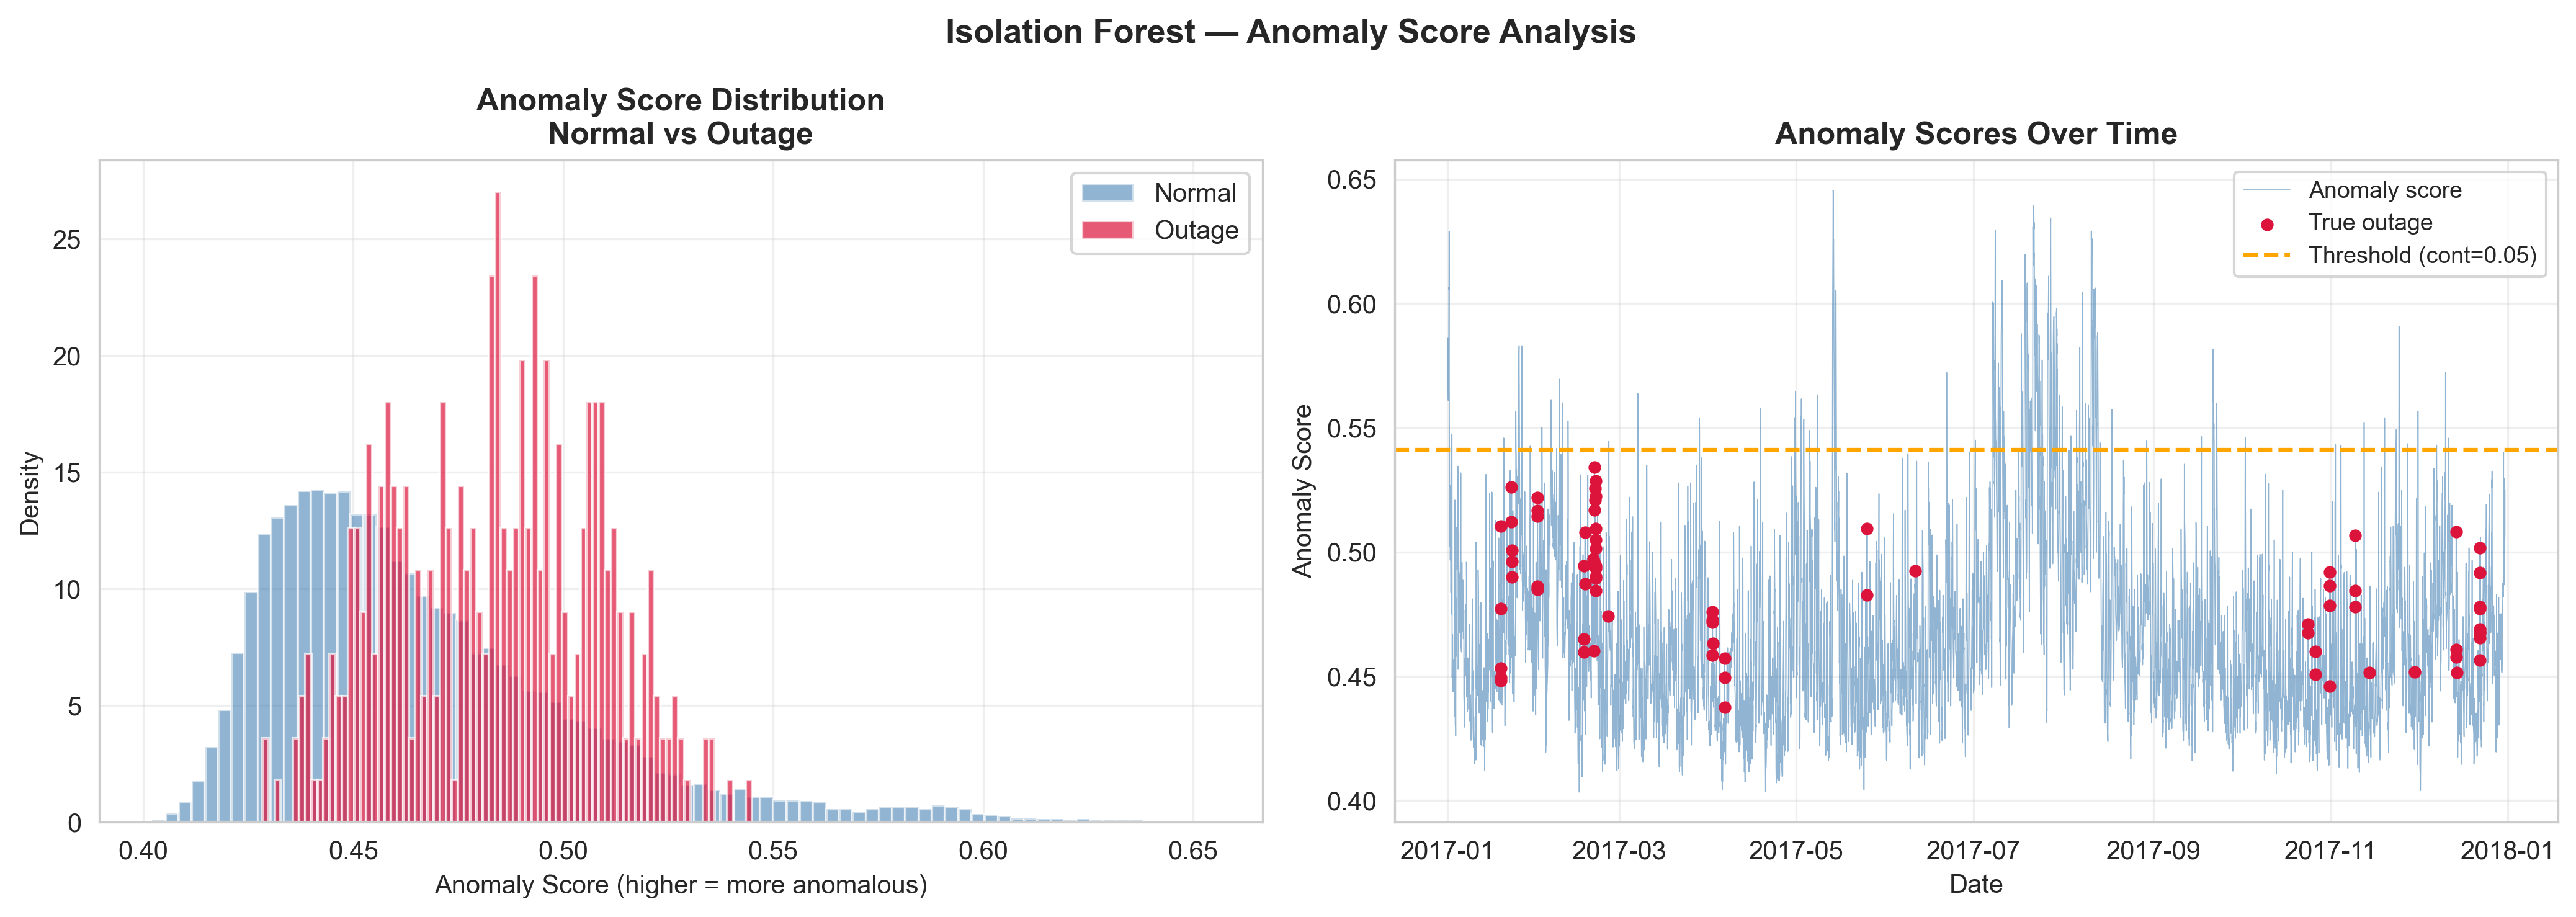
\includegraphics[width=\linewidth,height=2.4cm,keepaspectratio]{day4_plot2_anomaly_scores.png}
  \end{block}
\column{0.39\textwidth}
  \begin{block}{\faInfoCircle\ How It Works}
    \footnotesize
    \begin{enumerate}\setlength\itemsep{3pt}
      \item Randomly select a feature
      \item Random split between min/max
      \item Repeat until point is isolated
      \item \textbf{Anomalies} = isolated in \textbf{fewer splits}
      \item \textbf{Normal} = needs many splits
    \end{enumerate}
  \end{block}
  \vspace{3pt}
  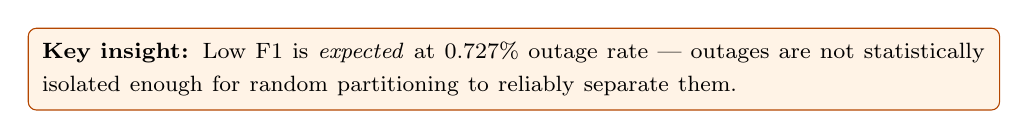
\begin{tikzpicture}
    \node[fill=WarnBg,draw=AccentOrange,rounded corners=3pt,
          inner sep=5pt,text width=\linewidth-4pt]{
      \footnotesize\textbf{Key insight:} Low F1 is \textit{expected} at 0.727\% outage rate --- outages are not statistically isolated enough for random partitioning to reliably separate them.
    };
  \end{tikzpicture}
\end{columns}
\end{frame}

%% SLIDE 12 ── LSTM AE ───────────────────────────────────────
\begin{frame}{LSTM Autoencoder --- Sequence-Level Detection}
\begin{columns}[t]
\column{0.55\textwidth}
  \begin{block}{Training Loss \& Detection Results}
    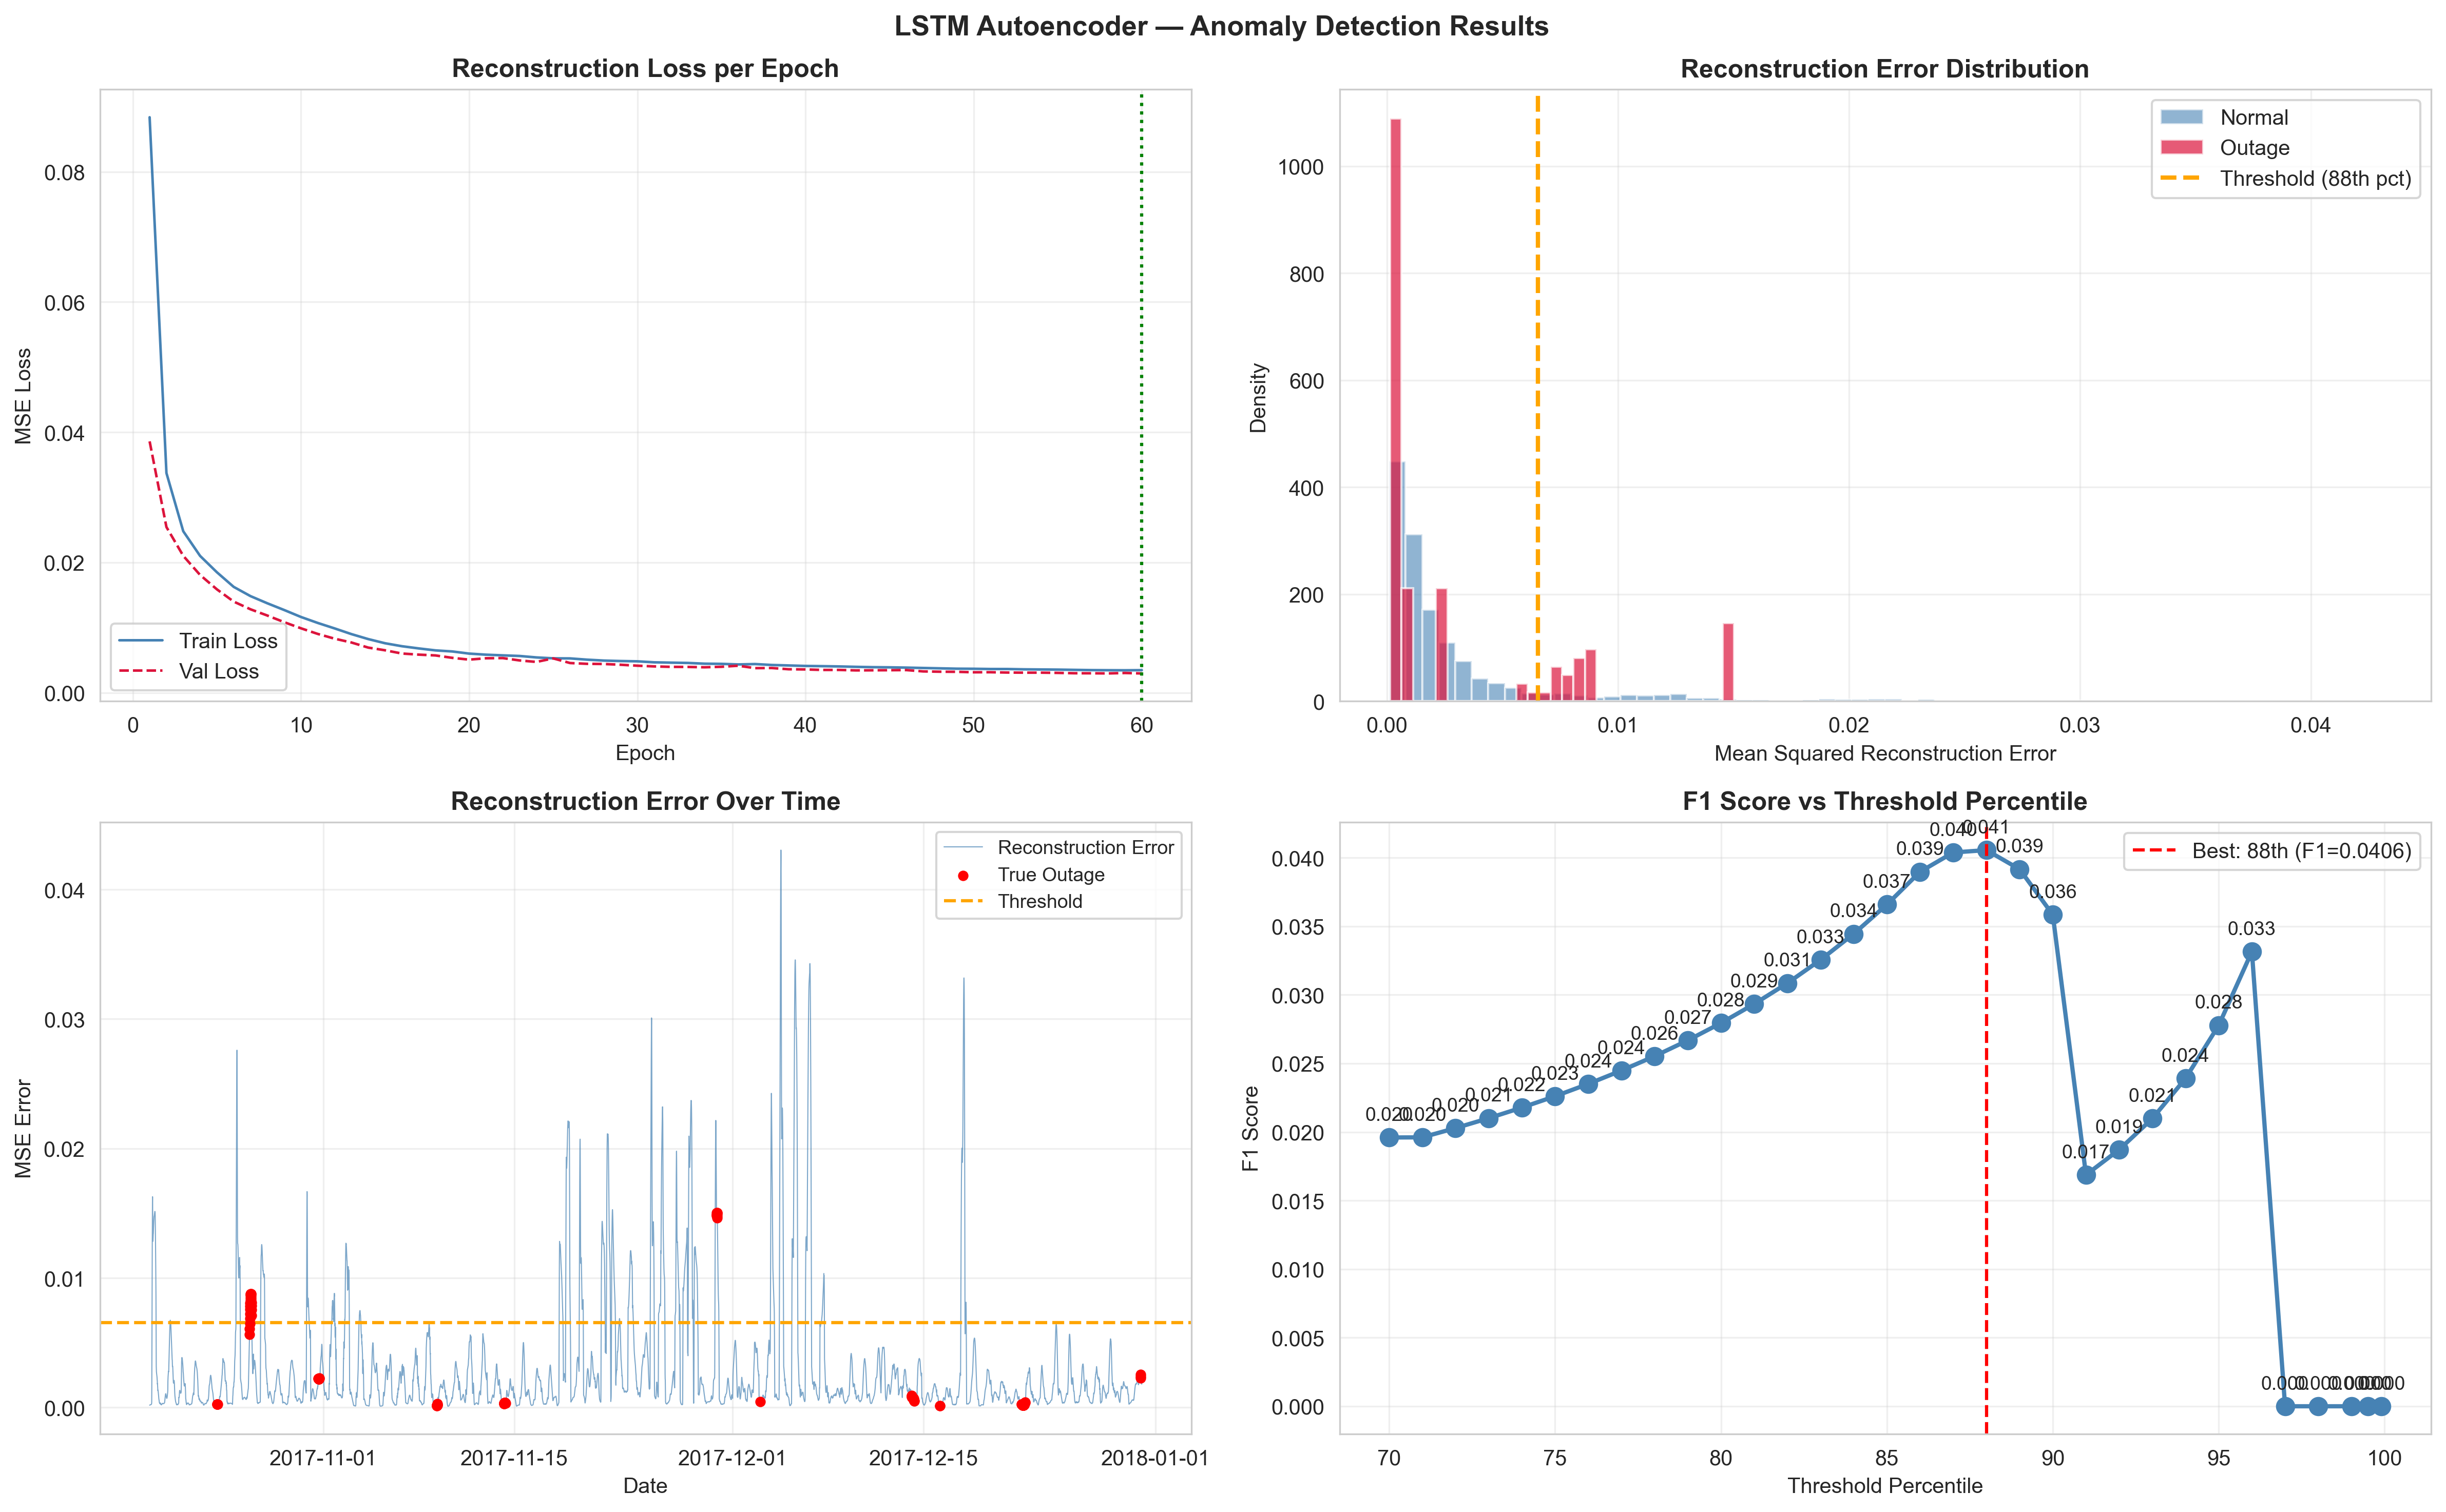
\includegraphics[width=\linewidth,height=4.2cm,keepaspectratio]{day4_plot9_lstm_ae_results.png}
  \end{block}
\column{0.42\textwidth}
  \begin{block}{\faNetworkWired\ Architecture}
    \footnotesize
    Window: 48 steps = 8 hrs\\
    Features: Zone 1/2/3, Temp, Humidity\\[3pt]
    \texttt{Input(48,5) $\to$ LSTM(64) $\to$}\\
    \texttt{LSTM(16) [Encoder] $\to$}\\
    \texttt{RepeatVector(48) $\to$}\\
    \texttt{LSTM(16) $\to$ LSTM(64) $\to$}\\
    \texttt{Dense(5) [Output]}
  \end{block}
  \vspace{3pt}
  \footnotesize
  \renewcommand{\arraystretch}{1.2}
  \begin{tabular}{@{}ll@{}}
    \toprule
    \textbf{Metric} & \textbf{Value}\\
    \midrule
    \rowcolor{RowAlt} Epochs      & 60\\
    Train Time   & 6.5 min\\
    \rowcolor{RowAlt} Best Val Loss & 0.002963\\
    F1 Score     & 0.0406\\
    \rowcolor{RowAlt} Recall      & 0.2258\\
    Precision    & 0.0223\\
    \bottomrule
  \end{tabular}
\end{columns}
\end{frame}

%% SLIDE 13 ── SHAP ──────────────────────────────────────────
\begin{frame}{SHAP --- Model Explainability}
\begin{columns}[t]
\column{0.49\textwidth}
  \begin{block}{Feature Importance (Bar)}
    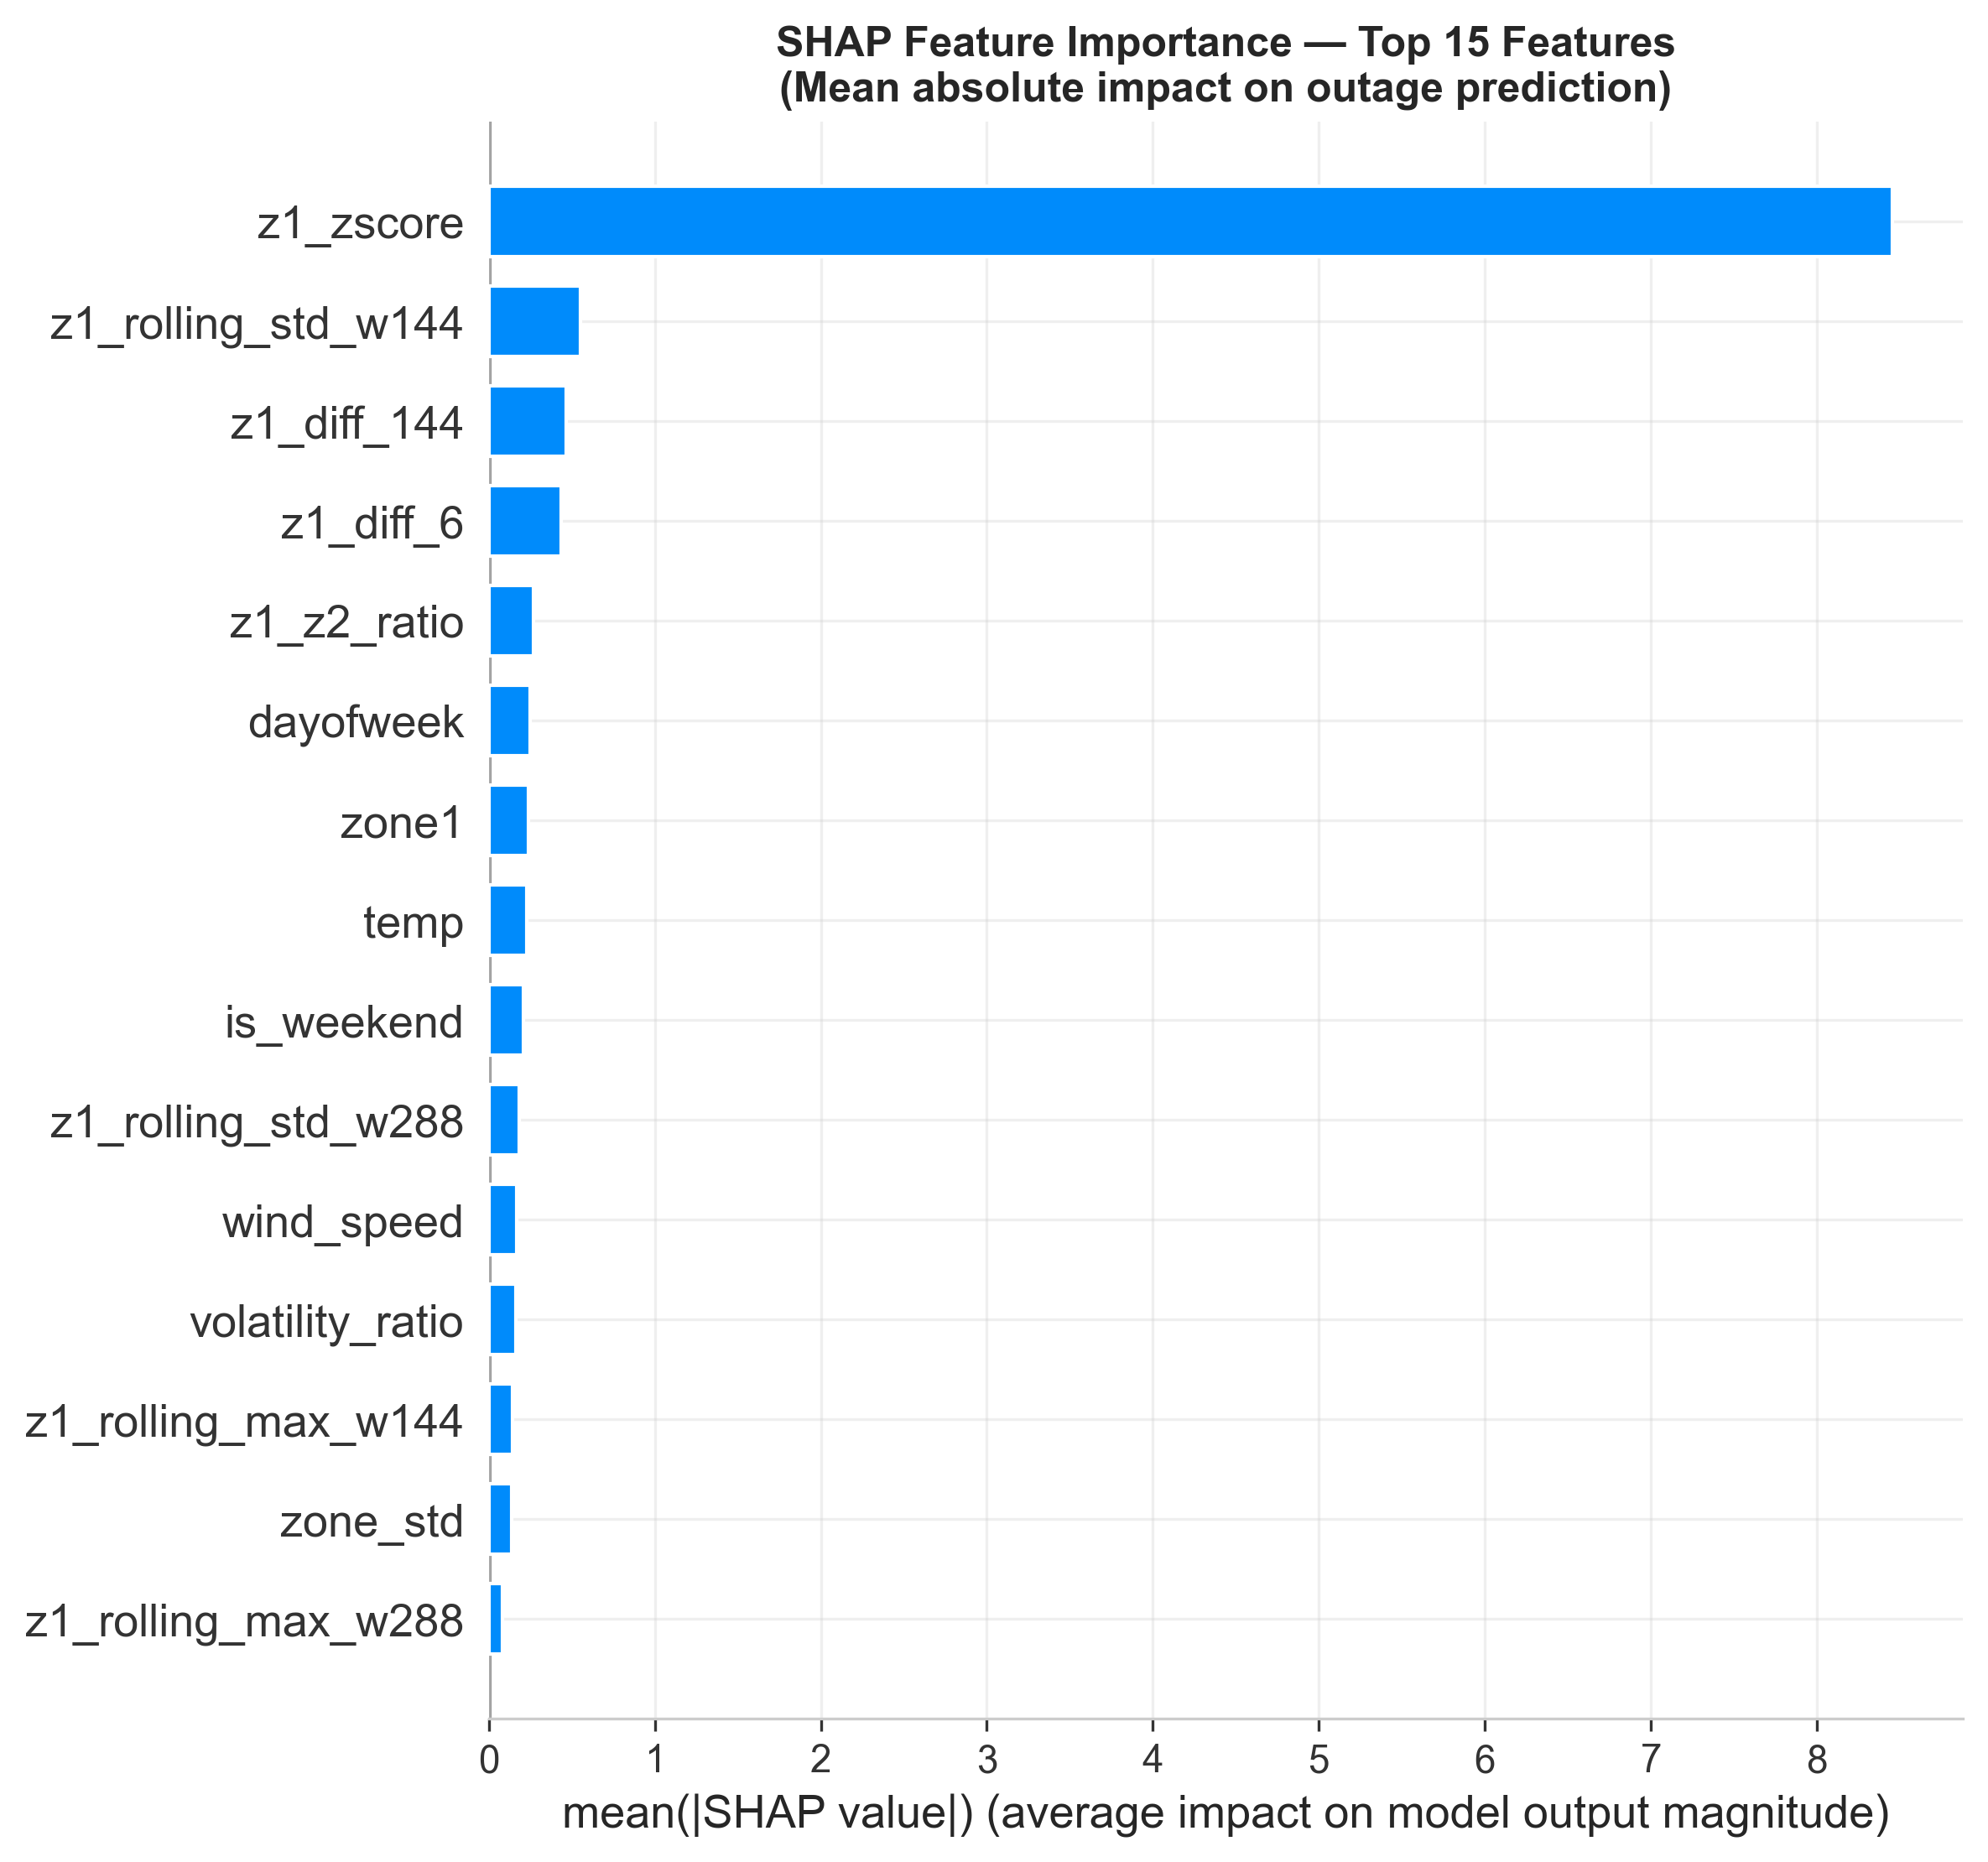
\includegraphics[width=\linewidth,height=3.8cm,keepaspectratio]{day4_plot5_shap_bar.png}
  \end{block}
\column{0.49\textwidth}
  \begin{block}{Beeswarm --- Impact Direction}
    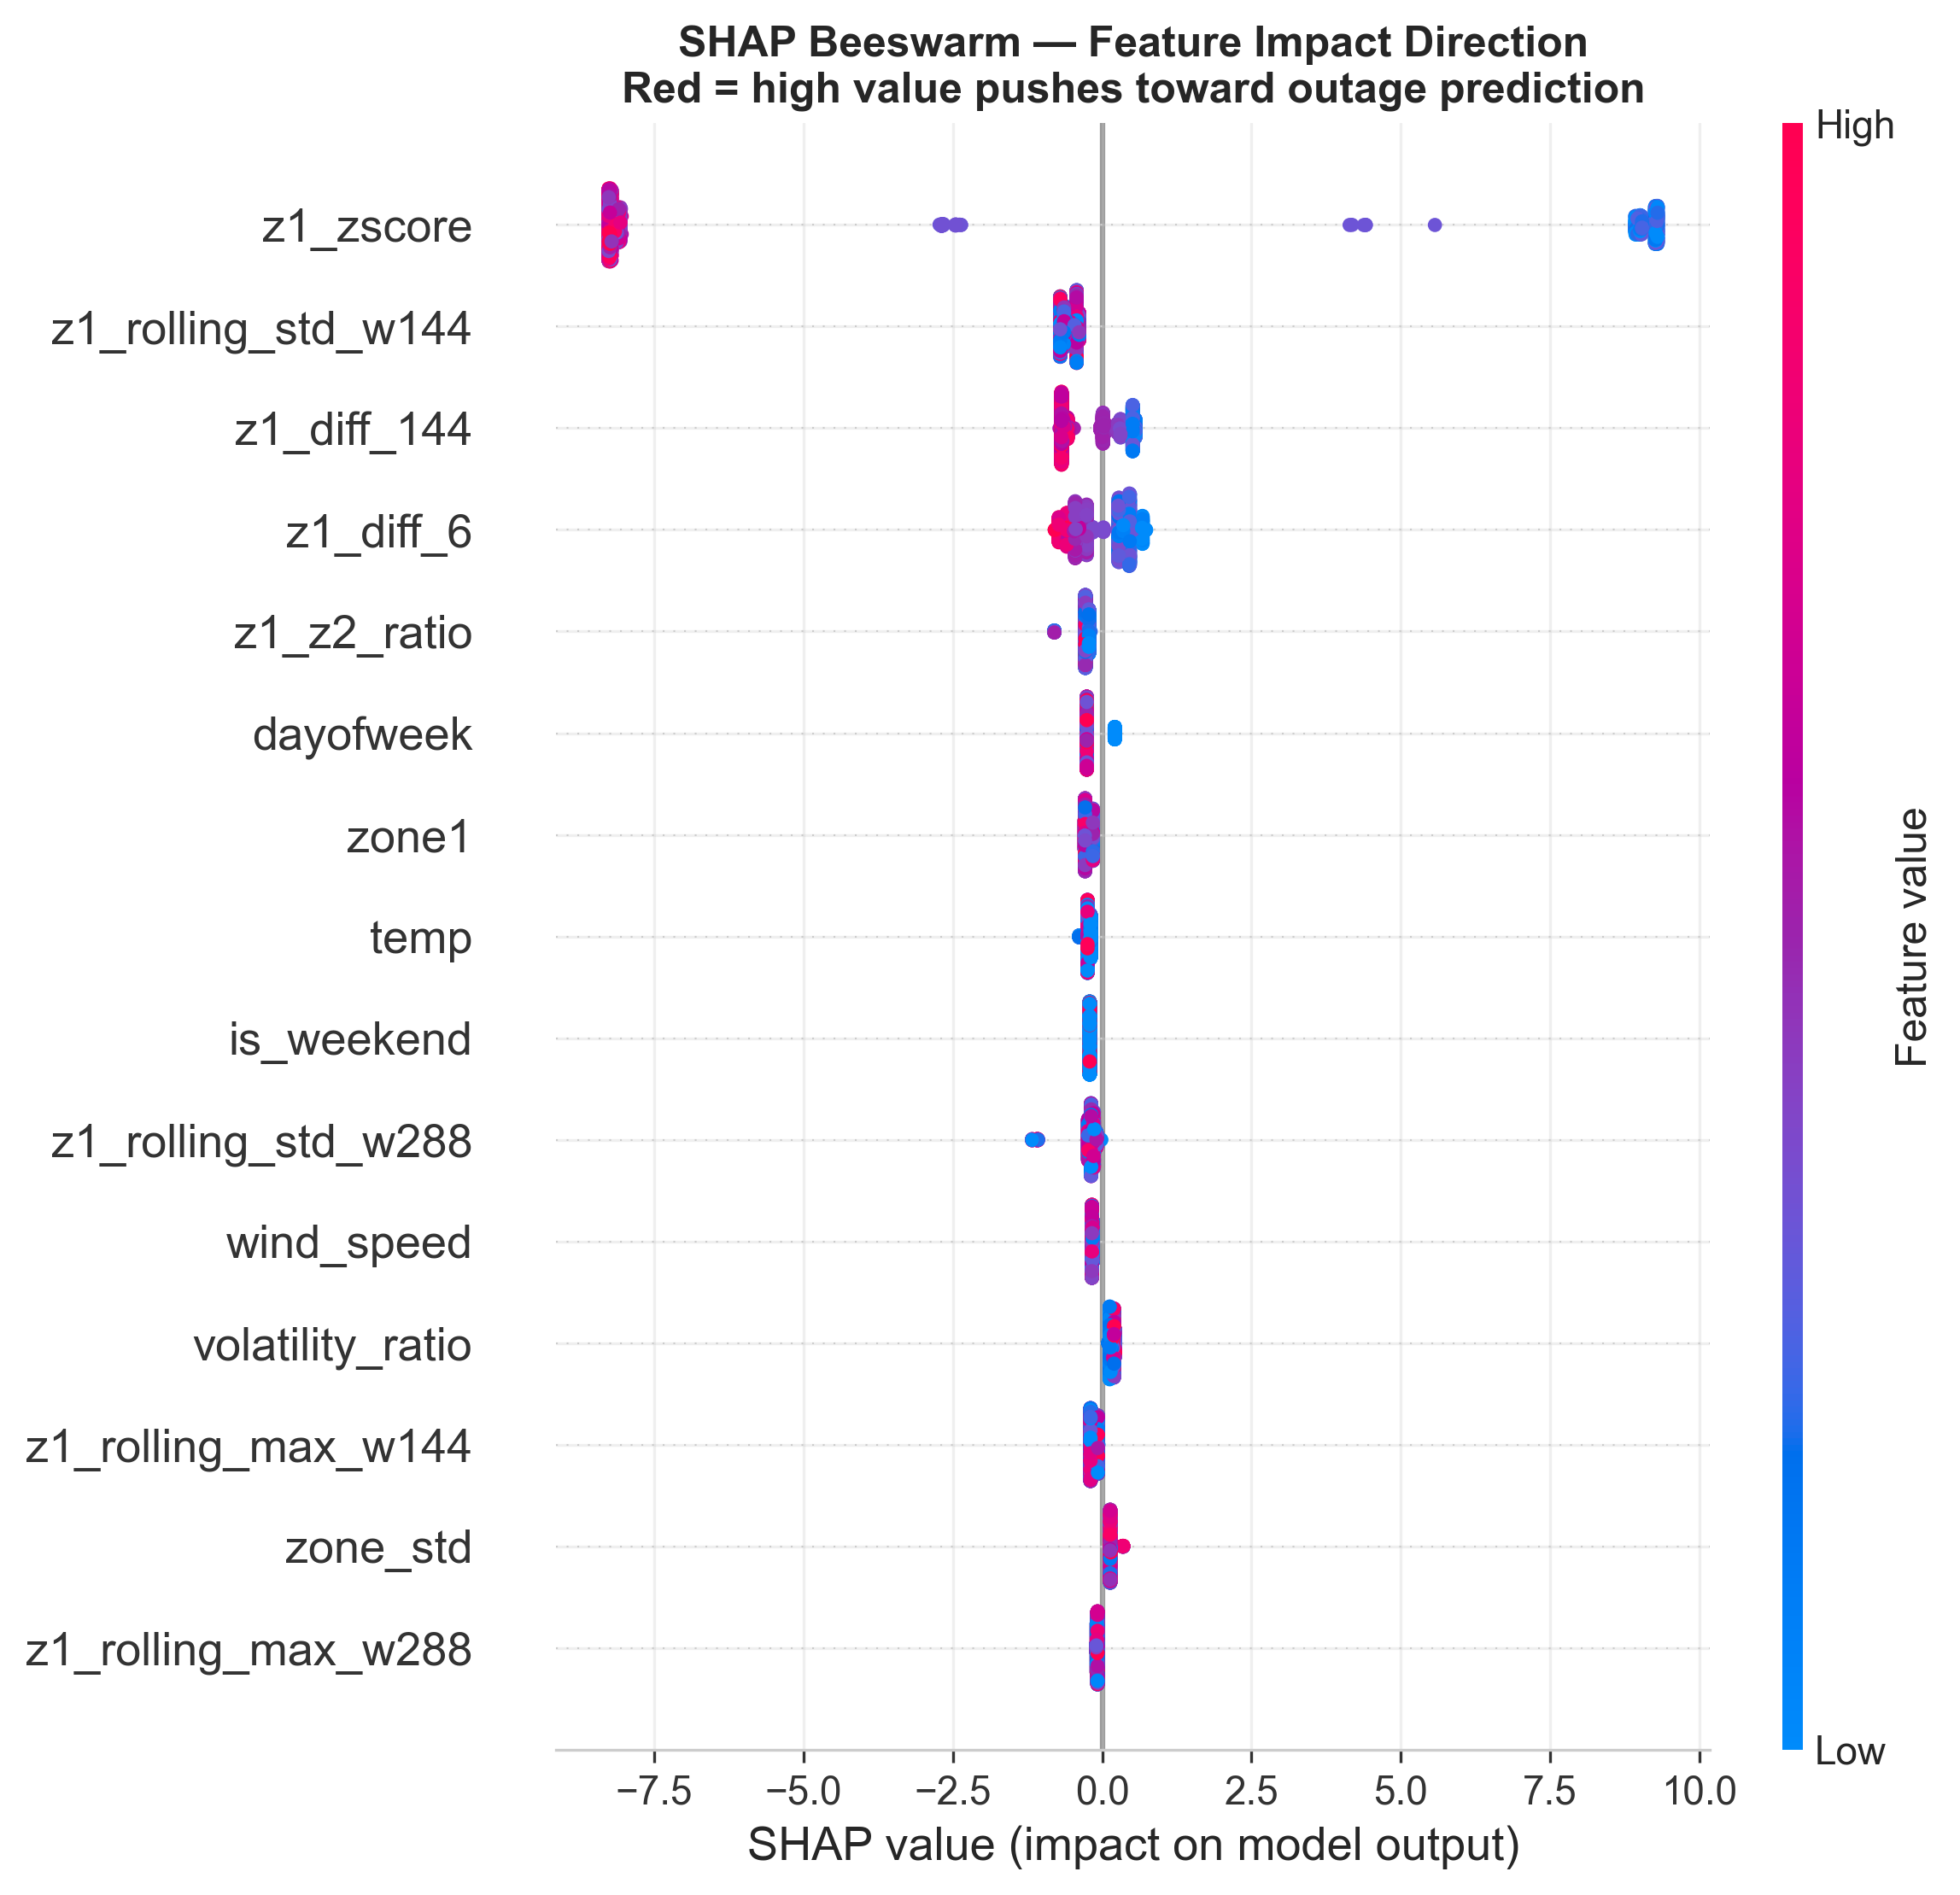
\includegraphics[width=\linewidth,height=3.8cm,keepaspectratio]{day4_plot6_shap_beeswarm.png}
  \end{block}
\end{columns}
\vspace{4pt}
\begin{columns}[t]
\column{0.49\textwidth}
  \chip{z1\_zscore}{PrimaryBlue}\ SHAP: 8.456 --- primary anomaly signal
\column{0.49\textwidth}
  \chip{z1\_rolling\_std\_w144}{AccentTeal}\ SHAP: 0.551 --- volatility before outage
\end{columns}
\end{frame}

%% SLIDE 14 ── SHAP WATERFALL ────────────────────────────────
\begin{frame}{SHAP Waterfall --- Single Outage Explained}
\begin{columns}[t]
\column{0.58\textwidth}
  \begin{block}{Why did the model flag this reading?}
    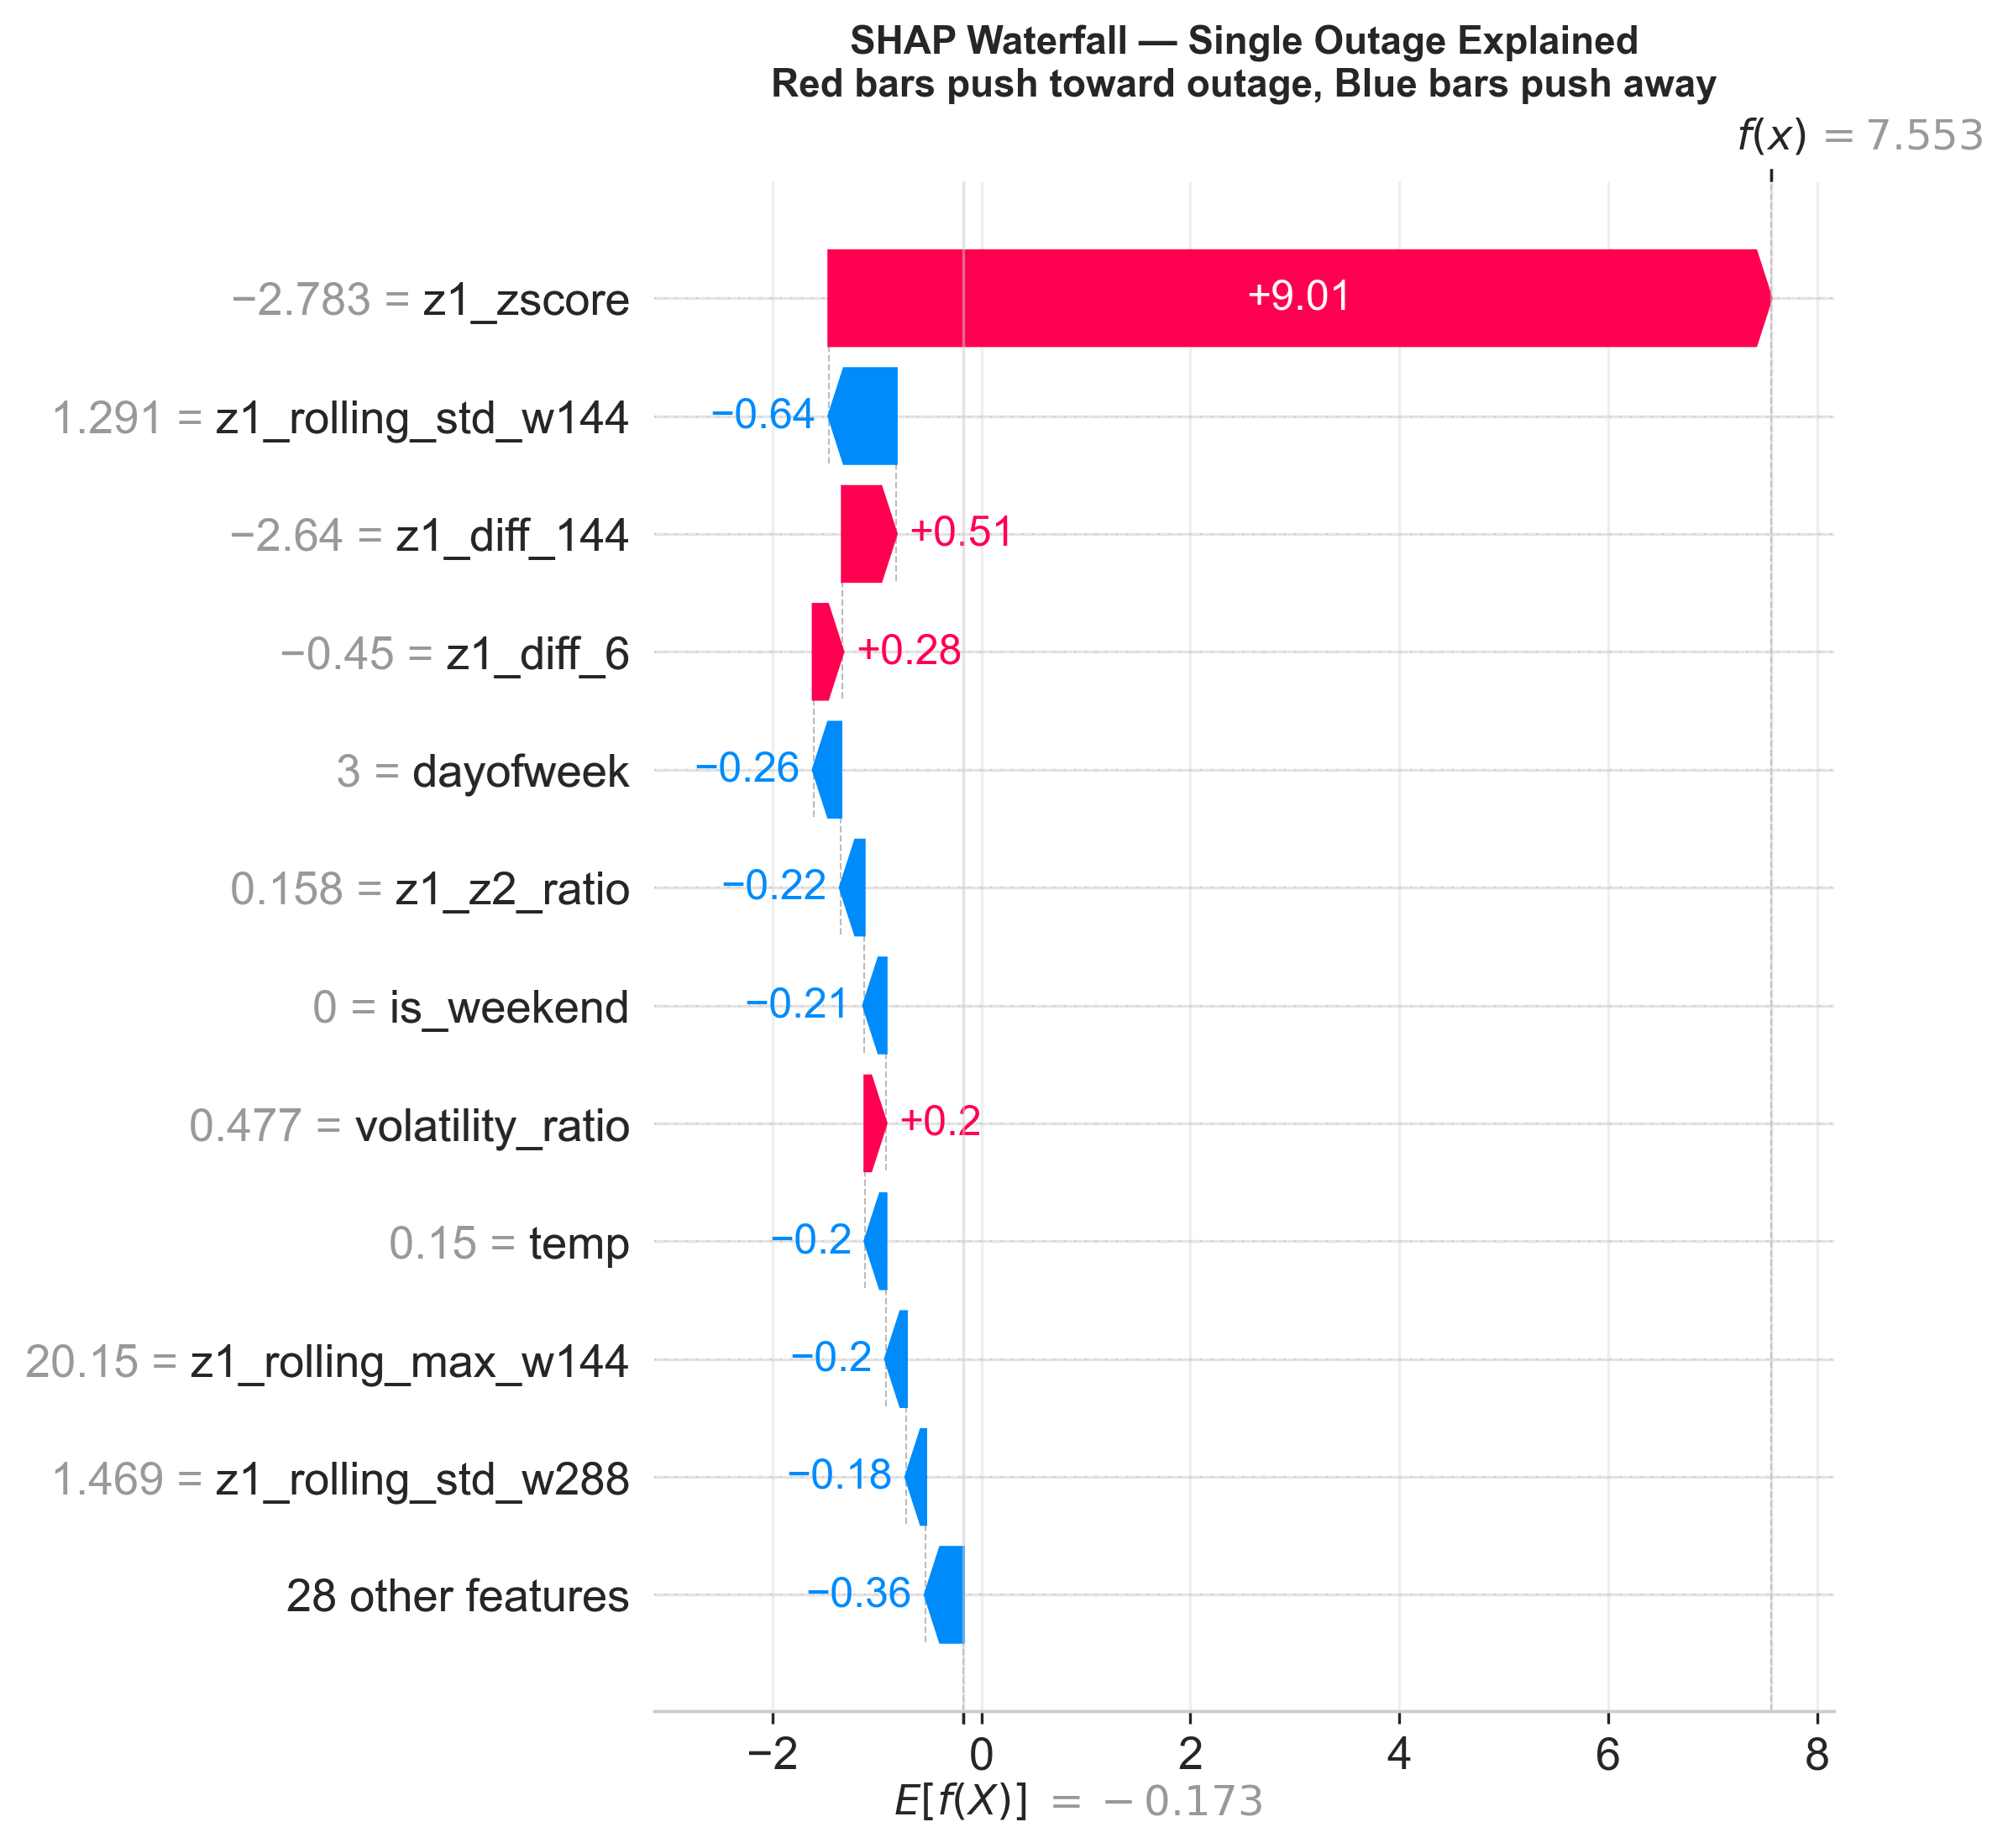
\includegraphics[width=\linewidth,height=4.8cm,keepaspectratio]{day4_plot7_shap_waterfall.png}
  \end{block}
\column{0.39\textwidth}
  \begin{exampleblock}{\faBook\ Interpretation}
    \footnotesize
    \begin{itemize}\setlength\itemsep{4pt}
      \item \textbf{Red bars} push toward outage prediction
      \item \textbf{Blue bars} push away from outage
      \item \texttt{z1\_zscore} dominates --- extreme deviation is the clearest signal
      \item SHAP = Shapley values from cooperative game theory
    \end{itemize}
  \end{exampleblock}
  \vspace{4pt}
  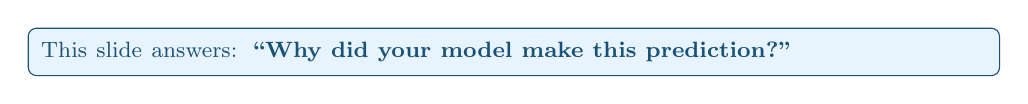
\begin{tikzpicture}
    \node[fill=CardBg,draw=PrimaryBlue,rounded corners=3pt,
          inner sep=5pt,text width=\linewidth-4pt]{
      \footnotesize\textcolor{PrimaryBlue}{This slide answers: \textbf{``Why did your model make this prediction?''}}
    };
  \end{tikzpicture}
\end{columns}
\end{frame}

%% SLIDE 15 ── RESULTS TABLE ─────────────────────────────────
\begin{frame}{Results --- Full Model Comparison}
\vspace{2pt}
\begin{center}
  \small
  \renewcommand{\arraystretch}{1.5}
  \begin{tabular}{@{}llccccc@{}}
    \toprule
    \textbf{Model} & \textbf{Type} & \textbf{F1} & \textbf{Precision} & \textbf{Recall} & \textbf{AUC}\\
    \midrule
    \rowcolor{GreenOk!10}
    XGBoost \faTrophy & Supervised & \textbf{0.9935} & \textbf{0.9870} & \textbf{1.0000} & \textbf{1.0000}\\
    Neural Network & Supervised & 0.9212 & 0.8539 & 1.0000 & 0.9999\\
    \rowcolor{RowAlt}
    LSTM Autoencoder & Unsupervised & 0.0406 & 0.0223 & 0.2258 & N/A\\
    Isolation Forest & Unsupervised & 0.0007 & 0.0004 & 0.0026 & N/A\\
    \bottomrule
  \end{tabular}
\end{center}
\vspace{3pt}
\begin{block}{All Models F1 / Precision / Recall Comparison}
  \centering
  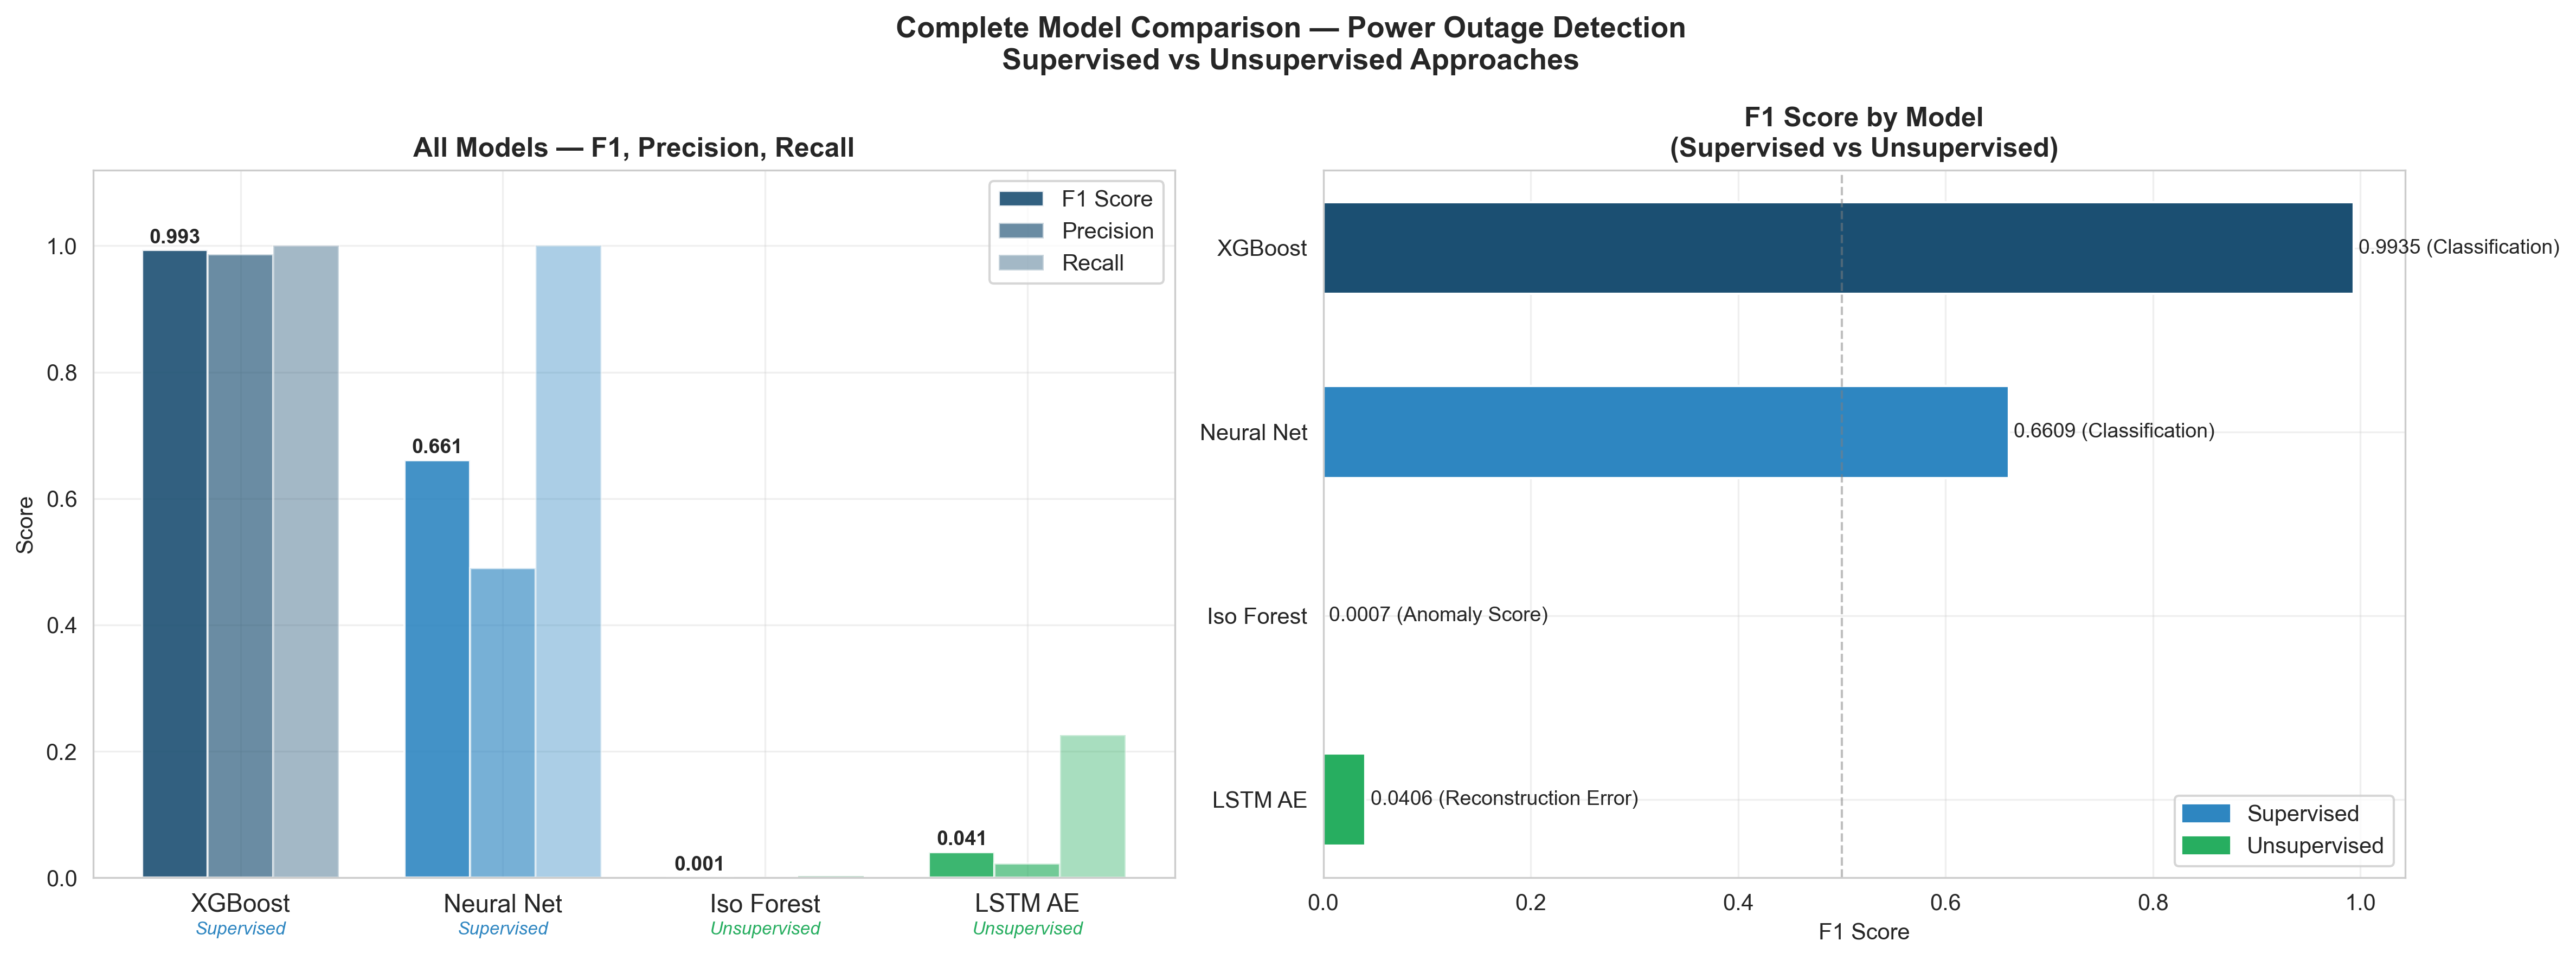
\includegraphics[width=0.82\linewidth,height=2.8cm,keepaspectratio]{day4_plot10_full_model_comparison.png}
\end{block}
\end{frame}

%% SLIDE 16 ── KEY FINDING ───────────────────────────────────
\begin{frame}{Key Finding --- Supervised vs.\ Unsupervised Gap}
\begin{columns}[t]
\column{0.48\textwidth}
  \begin{alertblock}{\faTimes\ Unsupervised Limitation}
    \footnotesize
    LSTM AE and Isolation Forest achieve F1 $<$ 0.05 because they receive \textbf{zero label information} during training. They cannot distinguish power outages from holidays, demand spikes, or weather events.
  \end{alertblock}
  \vspace{4pt}
  \begin{block}{\faCheck\ When to Use Each}
    \footnotesize
    \begin{itemize}\setlength\itemsep{3pt}
      \item \textbf{Supervised:} labels available, production deployment
      \item \textbf{Unsupervised:} no labels, first-pass screening, novel anomaly discovery
    \end{itemize}
  \end{block}
\column{0.48\textwidth}
  \begin{exampleblock}{\faKey\ Core Insight}
    \footnotesize
    The gap between supervised (F1: 0.9935) and unsupervised (F1: 0.0406) reveals that \textbf{label availability is the single most important factor} for outage detection on severely imbalanced time-series data.
  \end{exampleblock}
  \vspace{8pt}
  \centering
  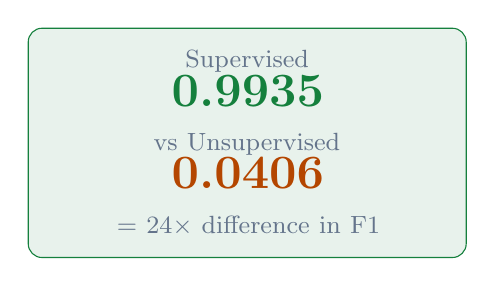
\begin{tikzpicture}
    \node[fill=GreenOk!10,draw=GreenOk,rounded corners=5pt,
          inner sep=8pt,align=center,text width=5cm]{
      {\small\textcolor{MutedText}{Supervised}}\\
      {\LARGE\bfseries\textcolor{GreenOk}{0.9935}}\\[4pt]
      {\small\textcolor{MutedText}{vs Unsupervised}}\\
      {\LARGE\bfseries\textcolor{AccentOrange}{0.0406}}\\[4pt]
      {\small\textcolor{MutedText}{= 24$\times$ difference in F1}}
    };
  \end{tikzpicture}
\end{columns}
\end{frame}

%% SLIDE 17 ── DASHBOARD ─────────────────────────────────────
\begin{frame}{Streamlit Dashboard --- Live Demo}
\begin{columns}[t]
\column{0.52\textwidth}
  \begin{block}{\faChartArea\ Dashboard Features}
    \footnotesize
    \begin{itemize}\setlength\itemsep{3pt}
      \item Live time-series with detected outages highlighted in orange
      \item Outage probability score panel with threshold line
      \item Three-zone comparison with outage regions shaded in red
      \item \textbf{Live prediction form:} input any sensor reading, get instant probability + gauge meter
      \item Model switching --- XGBoost, NN, Isolation Forest, LSTM AE
      \item Threshold slider to adjust detection sensitivity live
      \item Date range filter for time-window inspection
    \end{itemize}
  \end{block}
\column{0.45\textwidth}
  \begin{exampleblock}{\faCode\ Tech Stack}
    \footnotesize
    \begin{itemize}\setlength\itemsep{3pt}
      \item \textbf{Streamlit} --- web framework
      \item \textbf{Plotly} --- interactive charts
      \item \textbf{XGBoost} --- champion model
      \item \textbf{TensorFlow/Keras} --- LSTM AE
      \item \textbf{SHAP} --- explainability
      \item \textbf{scikit-learn} --- preprocessing
    \end{itemize}
  \end{exampleblock}
  \vspace{6pt}
  \centering
  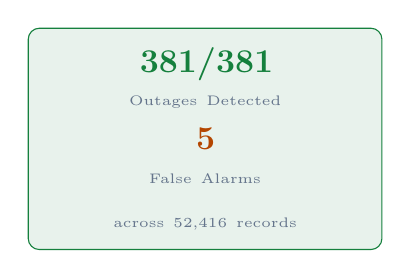
\begin{tikzpicture}
    \node[fill=GreenOk!10,draw=GreenOk,rounded corners=4pt,
          inner sep=7pt,align=center,text width=4.0cm]{
      {\large\bfseries\textcolor{GreenOk}{381/381}}\\
      {\tiny\textcolor{MutedText}{Outages Detected}}\\[4pt]
      {\large\bfseries\textcolor{AccentOrange}{5}}\\
      {\tiny\textcolor{MutedText}{False Alarms}}\\[4pt]
      {\tiny\textcolor{MutedText}{across 52,416 records}}
    };
  \end{tikzpicture}
\end{columns}
\end{frame}

%% SLIDE 18 ── CONCLUSION ────────────────────────────────────
\begin{frame}{Conclusion \& Future Work}
\begin{columns}[t]
\column{0.48\textwidth}
  \begin{exampleblock}{\faCheckCircle\ What We Achieved}
    \footnotesize
    \begin{itemize}\setlength\itemsep{3pt}
      \item XGBoost F1: \textbf{0.9935}, AUC: \textbf{1.0000}
      \item \textbf{381/381} outages detected, 5 false alarms
      \item \textbf{39 features} from 8 raw columns
      \item \textbf{20 training runs} across 4 NN architectures
      \item SHAP explainability for individual predictions
      \item 4 models across 2 paradigms compared
      \item Live Streamlit dashboard deployed
    \end{itemize}
  \end{exampleblock}
\column{0.48\textwidth}
  \begin{block}{\faRocket\ Future Work}
    \footnotesize
    \begin{itemize}\setlength\itemsep{3pt}
      \item Real-time streaming with Apache Kafka / MQTT
      \item LSTM/Transformer for supervised sequence classification
      \item Multi-class outage severity prediction
      \item Cloud deployment with SMS / email alerting
      \item Federated learning across utility providers
      \item Extension to additional city datasets
    \end{itemize}
  \end{block}
\end{columns}
\vspace{6pt}
\centering
{\large\textcolor{PrimaryBlue}{\textbf{Thank You\ \ |\ \ Questions?}}}
\end{frame}

\end{document}